\documentclass[12pt,a4paper]{article}
\usepackage[utf8]{inputenc}
\usepackage[T1]{fontenc}
\usepackage[spanish,es-tabla]{babel}
\usepackage{csquotes}
\usepackage{graphicx}
\usepackage{float}
\usepackage{geometry}
\usepackage{hyperref}
\usepackage{fancyhdr}
\usepackage{titlesec}
\usepackage{booktabs}
\usepackage{array}
\usepackage[table]{xcolor}
\definecolor{encabezado}{RGB}{208,219,232}
\definecolor{cebra}{gray}{0.92}
\definecolor{iteracion}{RGB}{198,222,245}
\definecolor{destacado}{RGB}{255,236,130}
\usepackage{mathptmx}
\usepackage{amsmath}
\usepackage{enumitem}
\usepackage{caption}
\usepackage{xurl}
\setlist{itemsep=1pt,topsep=3pt,parsep=0pt}
\captionsetup{font=small,labelfont=bf,position=bottom}
\setlength{\belowcaptionskip}{4pt}

\geometry{top=2.5cm, bottom=2.5cm, left=3cm, right=3cm}
\hypersetup{colorlinks=true, linkcolor=black, urlcolor=blue, citecolor=black}
\graphicspath{{../data/}{../outputs/}}

% bloque "Cómo leerla" de figuras y tablas de resultados
\newcommand{\comoleerla}[3]{%
  \begin{center}\footnotesize
  \begin{minipage}{0.94\linewidth}
  \begin{itemize}\setlength{\itemsep}{0pt}\setlength{\topsep}{2pt}%
    \setlength{\parsep}{0pt}
  \item \textbf{Estructura:} #1
  \item \textbf{Qué se ve:} #2
  \item \textbf{Por qué:} #3
  \end{itemize}
  \end{minipage}
  \end{center}}

% valores numéricos generados desde los .json
\newcommand{\PunoMejor}{\texttt{11111}}
\newcommand{\PunoX}{\ensuremath{31}}
\newcommand{\PunoAptitud}{\ensuremath{961}}
\newcommand{\PunoOptimo}{\ensuremath{961}}
\newcommand{\PunoMeseta}{\ensuremath{841}}
\newcommand{\PunoPrimeraGen}{\ensuremath{16}}
\newcommand{\PunoGenAntes}{\ensuremath{15}}
\newcommand{\PunoInicial}{\ensuremath{625}}
\newcommand{\PunoDistintosFinal}{\ensuremath{1}}
\newcommand{\PunoMaxDistintosMeseta}{\ensuremath{2}}
\newcommand{\PunoGenUniformes}{\ensuremath{9}}
\newcommand{\PunoProbHijo}{\ensuremath{0{,}0407}}
\newcommand{\PunoProbGen}{\ensuremath{0{,}1173}}
\newcommand{\PunoProbSinExito}{\ensuremath{0{,}0825}}
\newcommand{\PunoProbSinExitoPorc}{$8{,}3$\,\%}
\newcommand{\PunoProbGenPorc}{$11{,}7$\,\%}
\newcommand{\PunoProbHijoPorc}{$4{,}1$\,\%}
\newcommand{\PunoSuma}{\ensuremath{1118}}
\newcommand{\PunoProbMax}{\ensuremath{0{,}5590}}
\newcommand{\PdosExitos}{\ensuremath{5}}
\newcommand{\PdosTotal}{\ensuremath{9}}
\newcommand{\PdosProporcion}{$55{,}6$\,\%}
\newcommand{\PdosFallo}{\ensuremath{0{,}4444}}
\newcommand{\PdosFrac}{\ensuremath{5/9}}
\newcommand{\PdosFalloFrac}{\ensuremath{4/9}}
\newcommand{\PdosProbTres}{\ensuremath{0{,}9122}}
\newcommand{\PdosProbCinco}{\ensuremath{0{,}9827}}
\newcommand{\PdosProbUno}{\ensuremath{0{,}5556}}
\newcommand{\PdosProbDos}{\ensuremath{0{,}8025}}
\newcommand{\PtresEnergiaMaxima}{\ensuremath{4}}
\newcommand{\PtresDesdeFijo}{\ensuremath{31}}
\newcommand{\PtresMejor}{\ensuremath{0}}
\newcommand{\PtresEnergia}{\ensuremath{0}}
\newcommand{\PtresFinal}{\ensuremath{0}}
\newcommand{\PtresPeores}{\ensuremath{7}}
\newcommand{\PtresPropuestasPeores}{\ensuremath{88}}
\newcommand{\PtresIterMejor}{\ensuremath{5}}
\newcommand{\PtresIterSalida}{\ensuremath{6}}
\newcommand{\PtresPeorQueMejor}{\ensuremath{15}}
\newcommand{\PtresUltimoPeor}{\ensuremath{28}}
\newcommand{\PtresTempUltimoPeor}{\ensuremath{0{,}58}}
\newcommand{\PtresTempFinal}{\ensuremath{2{,}95\times10^{-4}}}
\newcommand{\PtresTempInicial}{\ensuremath{10{,}0}}
\newcommand{\PtresEnergiaInicial}{\ensuremath{25}}
\newcommand{\PtresEnergiaSalida}{\ensuremath{1}}
\newcommand{\PtresPeoresMitad}{\ensuremath{7}}
\newcommand{\PtresPropuestasMitad}{\ensuremath{38}}
\newcommand{\PtresPropuestasSegunda}{\ensuremath{50}}
\newcommand{\PcuatroBIni}{\ensuremath{0{,}5202}}
\newcommand{\PcuatroBFin}{\ensuremath{0{,}9974}}
\newcommand{\PcuatroBFrec}{\ensuremath{185}}
\newcommand{\PcuatroBPorc}{$92{,}5$\,\%}
\newcommand{\PcuatroBFer}{\ensuremath{81{,}92}}
\newcommand{\PcuatroBDep}{\ensuremath{1{,}67}}
\newcommand{\PcuatroBDos}{\ensuremath{0{,}6362}}
\newcommand{\PcuatroBCinco}{\ensuremath{0{,}8448}}
\newcommand{\PcuatroCIni}{\ensuremath{0{,}2926}}
\newcommand{\PcuatroCFin}{\ensuremath{0{,}0020}}
\newcommand{\PcuatroCFrec}{\ensuremath{10}}
\newcommand{\PcuatroCPorc}{$5{,}0$\,\%}
\newcommand{\PcuatroCFer}{\ensuremath{0{,}24}}
\newcommand{\PcuatroCDep}{\ensuremath{1{,}25}}
\newcommand{\PcuatroCDos}{\ensuremath{0{,}2780}}
\newcommand{\PcuatroCCinco}{\ensuremath{0{,}1197}}
\newcommand{\PcuatroDIni}{\ensuremath{0{,}1873}}
\newcommand{\PcuatroDFin}{\ensuremath{0{,}0006}}
\newcommand{\PcuatroDFrec}{\ensuremath{5}}
\newcommand{\PcuatroDPorc}{$2{,}5$\,\%}
\newcommand{\PcuatroDFer}{\ensuremath{0{,}11}}
\newcommand{\PcuatroDDep}{\ensuremath{1{,}00}}
\newcommand{\PcuatroDDos}{\ensuremath{0{,}0859}}
\newcommand{\PcuatroDCinco}{\ensuremath{0{,}0355}}
\newcommand{\PcuatroIterTodas}{\ensuremath{5}}
\newcommand{\PcuatroPrimeraB}{\ensuremath{4}}
\newcommand{\PcuatroPrimeraC}{\ensuremath{4}}
\newcommand{\PcuatroPrimeraD}{\ensuremath{2}}
\newcommand{\PcuatroUltimaC}{\ensuremath{3}}
\newcommand{\PcuatroUltimaD}{\ensuremath{4}}
\newcommand{\PcuatroPicoC}{\ensuremath{10{,}46}}
\newcommand{\PcuatroIterPicoC}{\ensuremath{3}}
\newcommand{\PcuatroDecisiones}{\ensuremath{200}}
\newcommand{\PcuatroIterPicoD}{\ensuremath{4}}
\newcommand{\PcuatroPesoB}{\ensuremath{0{,}2500}}
\newcommand{\PcuatroProbA}{\ensuremath{0{,}6024}}
\newcommand{\PcuatroProbAPorc}{$60{,}24$\,\%}
\newcommand{\PcuatroSumaPesos}{\ensuremath{0{,}415}}
\newcommand{\PcincoX}{\ensuremath{-1{,}848\times10^{-4}}}
\newcommand{\PcincoY}{\ensuremath{1{,}388\times10^{-5}}}
\newcommand{\PcincoF}{\ensuremath{3{,}434\times10^{-8}}}
\newcommand{\PcincoMaxFinal}{\ensuremath{1{,}46\times10^{-2}}}
\newcommand{\PcincoDist}{\ensuremath{1{,}853\times10^{-4}}}
\newcommand{\PcincoFInicial}{\ensuremath{7{,}760}}
\newcommand{\PcincoFUno}{\ensuremath{0{,}653}}
\newcommand{\PcincoDistMedia}{\ensuremath{3{,}567\times10^{-3}}}
\newcommand{\PcincoRapidez}{\ensuremath{8{,}701\times10^{-3}}}
\newcommand{\PcincoUltimaMejora}{\ensuremath{27}}
\newcommand{\PcincoSinMejora}{\ensuremath{3}}
\newcommand{\PcincoIteraciones}{\ensuremath{30}}
\newcommand{\PcincoReduccion}{\ensuremath{2{,}26\times10^{8}}}
\newcommand{\PcincoIterMenorUno}{\ensuremath{1}}
\newcommand{\PcincoIterMenorMilesima}{\ensuremath{14}}
\newcommand{\PcincoAptitudMilesima}{\ensuremath{3{,}26\times10^{-4}}}
\newcommand{\PcincoCuenta}{\ensuremath{19}}


\pagestyle{fancy}
\fancyhf{}
\fancyhead[L]{\small\nouppercase{\leftmark}}
\fancyhead[R]{\thepage}
\renewcommand{\headrulewidth}{0.4pt}
\setlength{\headheight}{14.5pt}
\setlength{\emergencystretch}{3em}

\titleformat{\section}{\normalfont\Large\bfseries}{\thesection}{1em}{}
\titleformat{\subsection}{\normalfont\large\bfseries}{\thesubsection}{1em}{}
\titleformat{\subsubsection}{\normalfont\normalsize\bfseries}{\thesubsubsection}{1em}{}

\begin{document}

\begin{titlepage}
\thispagestyle{empty}
\centering

\vspace*{0.5cm}

\includegraphics[width=0.30\textwidth]{sergio_logo.png}\\[0.4cm]

{\fontsize{13}{15}\selectfont\textbf{UNIVERSIDAD SERGIO ARBOLEDA}}\\[2.0cm]

{\fontsize{14}{17}\selectfont\textbf{PARCIAL 2: ALGORITMOS EVOLUTIVOS,\\
GENÉTICOS, ASCENSO DE COLINAS,\\
TEMPLE SIMULADO, ACO Y PSO}}\\[0.6cm]
{\fontsize{12}{14}\selectfont Fundamentos de Inteligencia Artificial}\\[2.5cm]

{\fontsize{12}{14}\selectfont\textbf{Inteligencia Artificial (SIST5036)}}\\[1.5cm]

{\fontsize{12}{14}\selectfont\textbf{Camilo Andrés Díaz García}\\[0.2cm]
\textbf{Juan David Andradé Gómez}\\[0.2cm]
\textbf{Mario Jiménez López}}\\[1.2cm]

{\fontsize{12}{14}\selectfont Profesor: Joaquín F. Sánchez}

\vfill

\begin{center}
    \textit{Universidad Sergio Arboleda}\\
    \textit{Facultad de Sistemas e Ingeniería}\\
    \textit{Bogotá, octubre de 2026}
\end{center}

\end{titlepage}

\newpage
\tableofcontents
\newpage

%=====================================================================
\section{Punto 1. Algoritmos evolutivos y algoritmos genéticos}

Se maximiza $f(x)=x^2$ con $x\in\{0,\dots,31\}$. Cada solución es un
cromosoma de cinco bits. La población inicial es
$P=\{\texttt{00101},\texttt{01100},\texttt{10010},\texttt{11001}\}$.

\subsection{Parte A: componente matemático y conceptual}

\noindent\textbf{1. Decodificación y aptitud.} Cada cromosoma se lee como un
número binario. Por ejemplo,
$\texttt{00101}=0\cdot16+0\cdot8+1\cdot4+0\cdot2+1\cdot1=5$ y su aptitud es
$5^2=25$. Los demás se calculan igual (Tabla~\ref{tab:p1a-ruleta}).

\noindent\textbf{2. Probabilidad de ruleta.} Cada individuo recibe una
fracción de la ruleta proporcional a su aptitud. La suma de las aptitudes es
\PunoSuma{}. El individuo \texttt{11001} tiene la mayor probabilidad
(\PunoProbMax{}) porque su aptitud es la más alta.

\begin{table}[H]
\centering
\small
\setlength{\tabcolsep}{6pt}
\renewcommand{\arraystretch}{1.15}
\begin{tabular}{|c|c|c|c|}
\hline
\textbf{Cromosoma} & \textbf{$x$} & \textbf{$f(x)$} & \textbf{Probabilidad de ruleta} \\
\hline
\texttt{00101} & $5$ & $25$ & $0{,}0224$ \\
\hline
\texttt{01100} & $12$ & $144$ & $0{,}1288$ \\
\hline
\texttt{10010} & $18$ & $324$ & $0{,}2898$ \\
\hline
\texttt{11001} & $25$ & $625$ & $0{,}5590$ \\
\hline
Suma &  & $1118$ & $1{,}0000$ \\
\hline
\end{tabular}
\caption{Decodificación, aptitud y probabilidad de selección por ruleta de la población inicial.}
\label{tab:p1a-ruleta}
\end{table}


\noindent\textbf{3. Cruce.} Los padres son \texttt{01100} y \texttt{11001}.
Se cortan después del segundo bit: \texttt{01|100} y \texttt{11|001}. Cada
descendiente toma el inicio de un padre y el final del otro:
\texttt{01001} y \texttt{11100}.

\noindent\textbf{4. Mutación.} Al invertir el último bit de \texttt{01001}
se obtiene \texttt{01000}. Su valor es $x=8$ y su aptitud baja de $81$ a
$64$ (Tabla~\ref{tab:p1a-cruce}).

\begin{table}[H]
\centering
\small
\setlength{\tabcolsep}{6pt}
\renewcommand{\arraystretch}{1.15}
\begin{tabular}{|c|c|c|c|}
\hline
\textbf{Individuo} & \textbf{Cromosoma} & \textbf{$x$} & \textbf{$f(x)$} \\
\hline
Padre 1 & \texttt{01100} & $12$ & $144$ \\
\hline
Padre 2 & \texttt{11001} & $25$ & $625$ \\
\hline
Descendiente 1 & \texttt{01001} & $9$ & $81$ \\
\hline
Descendiente 2 & \texttt{11100} & $28$ & $784$ \\
\hline
Descendiente 1 mutado & \texttt{01000} & $8$ & $64$ \\
\hline
\end{tabular}
\caption{Cruce de un punto tras el segundo bit y mutación del último bit del primer descendiente.}
\label{tab:p1a-cruce}
\end{table}


\noindent\textbf{5. Explicación breve.}
\begin{itemize}
  \item \textbf{Evolutivo y genético.} Un algoritmo evolutivo mejora una
  población de soluciones por selección y variación a lo largo de
  generaciones. El algoritmo genético es una familia dentro de los
  evolutivos: representa cada solución como un cromosoma y usa selección,
  cruce y mutación.
  \item \textbf{Selección, cruce y mutación.} La selección decide quiénes se
  reproducen y favorece a los de mayor aptitud. El cruce combina material de
  dos padres para probar soluciones nuevas. La mutación cambia bits al azar
  y evita que la población se quede sin variedad.
  \item \textbf{Mutación útil aunque empeore.} Un cambio que baja la
  aptitud inmediata puede introducir un valor que ya no existe en la
  población. Un dato de este problema lo muestra: el cuarto bit vale $1$
  solo en \texttt{10010}. Si ese cromosoma desaparece, ningún cruce puede
  devolver ese bit, porque el cruce solo mezcla bits que ya existen. El
  óptimo \texttt{11111} no se obtiene con un solo cruce entre los cuatro
  cromosomas iniciales (comprobado por código). Con cruces repetidos sí es
  alcanzable, pero solo mientras \texttt{10010} siga en la población. Cuando
  se pierde, solo la mutación puede recuperar ese bit. La ejecución de la
  parte B lo confirma (Sección~\ref{sec:p1-interpretacion}).
\end{itemize}

\subsection{Parte B: implementación en Python}

\subsubsection{Decisiones de implementación}

\begin{table}[H]
\centering\small
\renewcommand{\arraystretch}{1.15}
\begin{tabular}{|l|>{\raggedright\arraybackslash}p{9.6cm}|}
\hline
\textbf{Aspecto} & \textbf{Supuesto adoptado} \\ \hline
Generador & \texttt{random.Random(42)}, creado una sola vez al inicio de
\texttt{algoritmo\_genetico}. \\ \hline
Nueva generación & El mejor individuo pasa sin cambios (elitismo; en un
empate se conserva el primero). Los otros tres se generan por ruleta, cruce
y mutación. \\ \hline
Ruleta & Con reemplazo: los dos padres pueden ser el mismo individuo. Usa un
número \texttt{random()} multiplicado por la suma de aptitudes y recorre el
acumulado. \\ \hline
Cruce & Una llamada \texttt{random()} decide si ocurre ($p<0{,}8$). Si ocurre,
\texttt{randint(1, 4)} fija el punto. Si no, los hijos son copias de los
padres. \\ \hline
Mutación & Cinco llamadas \texttt{random()} por hijo, una por bit, de
izquierda a derecha. Se invierte el bit si el número es menor que
$0{,}05$. \\ \hline
Descendientes & Se producen en pares. Como faltan tres, el segundo par
aporta un solo hijo y el sobrante se descarta antes de mutarlo, sin consumir
llamadas. \\ \hline
Orden por par & Padre 1, padre 2, decisión de cruce, punto de cruce,
mutación del hijo 1 y mutación del hijo 2. \\ \hline
Historial & Mejor aptitud en la generación 0 (población inicial) y tras cada
una de las 20 generaciones: 21 valores. \\ \hline
\end{tabular}
\caption{Decisiones de implementación del punto 1.}
\label{tab:p1-decisiones}
\end{table}

\subsubsection{Resultados}

\begin{table}[H]
\centering
\small
\setlength{\tabcolsep}{6pt}
\renewcommand{\arraystretch}{1.15}
\begin{tabular}{|c|c|c|c|c|}
\hline
\textbf{Mejor cromosoma} & \textbf{$x$} & \textbf{Aptitud} & \textbf{Máximo posible} & \textbf{Óptimo hallado} \\
\hline
\texttt{11111} & $31$ & $961$ & $961$ & Sí \\
\hline
\end{tabular}
\caption{Mejor individuo de la población final (generación 20).}
\label{tab:p1b-resumen}
\end{table}

\comoleerla
{una fila con el mejor individuo de la población final y el máximo teórico.}
{el cromosoma \PunoMejor{}, $x=\PunoX$ y aptitud \PunoAptitud{}, igual al
máximo posible \PunoOptimo{}.}
{permite comparar de inmediato lo hallado con el óptimo global.}

\begin{table}[H]
\centering
\footnotesize
\setlength{\tabcolsep}{4pt}
\renewcommand{\arraystretch}{1.15}
\begin{tabular}{|c|c|c|c|c|c|}
\hline
\textbf{Gen.} & \textbf{Mejor aptitud} & \textbf{Gen.} & \textbf{Mejor aptitud} & \textbf{Gen.} & \textbf{Mejor aptitud} \\
\hline
$0$ & $625$ & $7$ & $841$ & $14$ & $841$ \\
\hline
$1$ & $841$ & $8$ & $841$ & $15$ & $841$ \\
\hline
$2$ & $841$ & $9$ & $841$ & $16$ & $961$ \\
\hline
$3$ & $841$ & $10$ & $841$ & $17$ & $961$ \\
\hline
$4$ & $841$ & $11$ & $841$ & $18$ & $961$ \\
\hline
$5$ & $841$ & $12$ & $841$ & $19$ & $961$ \\
\hline
$6$ & $841$ & $13$ & $841$ & $20$ & $961$ \\
\hline
\end{tabular}
\caption{Historial de la mejor aptitud por generación (la generación 0 es la población inicial).}
\label{tab:p1b-historial}
\end{table}

\comoleerla
{tres bloques de columnas (generación y mejor aptitud) leídos de arriba hacia
abajo y de izquierda a derecha.}
{la aptitud parte en \PunoInicial{}, sube a \PunoMeseta{} en la generación
$1$, se mantiene hasta la generación \PunoGenAntes{} y llega a \PunoOptimo{}
en la generación \PunoPrimeraGen{}. Nunca baja.}
{el elitismo conserva siempre al mejor, así que la mejor aptitud no puede
decrecer.}

\begin{table}[H]
\centering
\footnotesize
\setlength{\tabcolsep}{3pt}
\renewcommand{\arraystretch}{1.15}
\begin{tabular}{|c|l|c|c|l|c|}
\hline
\rowcolor{encabezado}\textbf{Gen.} & \textbf{Población} & \textbf{Distintos} & \textbf{Gen.} & \textbf{Población} & \textbf{Distintos} \\
\hline
\cellcolor{destacado}{\bfseries\boldmath $0$} & \cellcolor{destacado}\texttt{00101} \texttt{01100} \texttt{10010} \texttt{11001} & \cellcolor{destacado}$4$ & \cellcolor{iteracion}{\bfseries\boldmath $11$} & \texttt{11101} \texttt{11101} \texttt{11001} \texttt{11101} & $2$ \\
\hline
\cellcolor{iteracion}{\bfseries\boldmath $1$} & \cellcolor{cebra}\texttt{11001} \texttt{11100} \texttt{11001} \texttt{11101} & \cellcolor{cebra}$3$ & \cellcolor{iteracion}{\bfseries\boldmath $12$} & \cellcolor{cebra}\texttt{11101} \texttt{11101} \texttt{11101} \texttt{11101} & \cellcolor{cebra}$1$ \\
\hline
\cellcolor{iteracion}{\bfseries\boldmath $2$} & \texttt{11101} \texttt{11100} \texttt{11001} \texttt{11101} & $3$ & \cellcolor{iteracion}{\bfseries\boldmath $13$} & \texttt{11101} \texttt{11101} \texttt{11101} \texttt{11101} & $1$ \\
\hline
\cellcolor{iteracion}{\bfseries\boldmath $3$} & \cellcolor{cebra}\texttt{11101} \texttt{11101} \texttt{11101} \texttt{11101} & \cellcolor{cebra}$1$ & \cellcolor{iteracion}{\bfseries\boldmath $14$} & \cellcolor{cebra}\texttt{11101} \texttt{11101} \texttt{11101} \texttt{11101} & \cellcolor{cebra}$1$ \\
\hline
\cellcolor{iteracion}{\bfseries\boldmath $4$} & \texttt{11101} \texttt{11101} \texttt{11101} \texttt{11101} & $1$ & \cellcolor{iteracion}{\bfseries\boldmath $15$} & \texttt{11101} \texttt{10101} \texttt{11101} \texttt{11101} & $2$ \\
\hline
\cellcolor{iteracion}{\bfseries\boldmath $5$} & \cellcolor{cebra}\texttt{11101} \texttt{11101} \texttt{01101} \texttt{01101} & \cellcolor{cebra}$2$ & \cellcolor{destacado}{\bfseries\boldmath $16$} & \cellcolor{destacado}\texttt{11101} \texttt{11101} \texttt{11111} \texttt{01101} & \cellcolor{destacado}$3$ \\
\hline
\cellcolor{iteracion}{\bfseries\boldmath $6$} & \texttt{11101} \texttt{11101} \texttt{01001} \texttt{11101} & $2$ & \cellcolor{iteracion}{\bfseries\boldmath $17$} & \texttt{11111} \texttt{00101} \texttt{11101} \texttt{01111} & $4$ \\
\hline
\cellcolor{iteracion}{\bfseries\boldmath $7$} & \cellcolor{cebra}\texttt{11101} \texttt{11101} \texttt{11101} \texttt{11101} & \cellcolor{cebra}$1$ & \cellcolor{iteracion}{\bfseries\boldmath $18$} & \cellcolor{cebra}\texttt{11111} \texttt{11111} \texttt{01111} \texttt{11111} & \cellcolor{cebra}$2$ \\
\hline
\cellcolor{iteracion}{\bfseries\boldmath $8$} & \texttt{11101} \texttt{11101} \texttt{11101} \texttt{11101} & $1$ & \cellcolor{iteracion}{\bfseries\boldmath $19$} & \texttt{11111} \texttt{01101} \texttt{01111} \texttt{11111} & $3$ \\
\hline
\cellcolor{iteracion}{\bfseries\boldmath $9$} & \cellcolor{cebra}\texttt{11101} \texttt{11101} \texttt{11101} \texttt{11101} & \cellcolor{cebra}$1$ & \cellcolor{iteracion}{\bfseries\boldmath $20$} & \cellcolor{cebra}\texttt{11111} \texttt{11111} \texttt{11111} \texttt{11111} & \cellcolor{cebra}$1$ \\
\hline
\cellcolor{iteracion}{\bfseries\boldmath $10$} & \texttt{11101} \texttt{01101} \texttt{11101} \texttt{11101} & $2$ &  &  &  \\
\hline
\end{tabular}
\caption{Población de cada generación y número de cromosomas distintos. En la tabla, el fondo azul marca la columna de generación; el gris claro alterna las filas; el fondo amarillo, con el número en negrita, señala la generación 0 (población inicial) y la generación 16 (primera en que aparece \texttt{11111}).}
\label{tab:p1b-poblaciones}
\end{table}

\comoleerla
{dos bloques de columnas con la generación, los cuatro cromosomas y cuántos
son distintos.}
{entre las generaciones $3$ y \PunoGenAntes{} hay como máximo
\PunoMaxDistintosMeseta{} cromosomas distintos. Entre las generaciones $1$ y \PunoGenAntes{} ningún individuo tiene
el cuarto bit en $1$. En la generación \PunoPrimeraGen{} aparece
\texttt{11111}.}
{muestra la pérdida de diversidad y el origen del óptimo, que solo pudo venir
de una mutación.}

\begin{figure}[H]
\centering
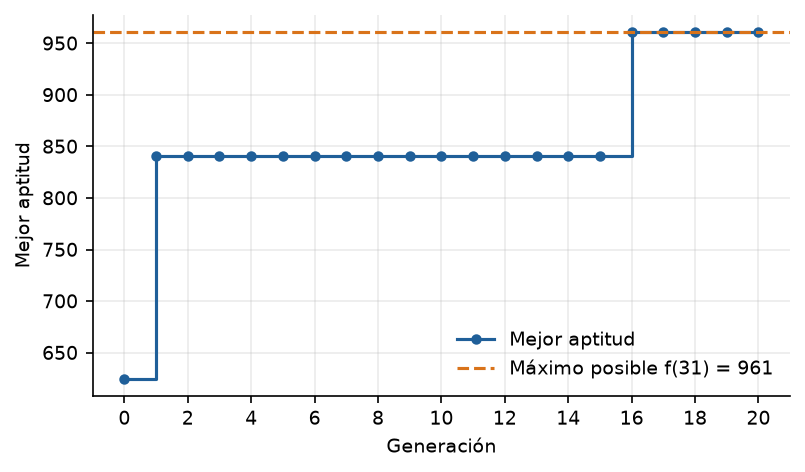
\includegraphics[width=0.85\textwidth]{p1_historial.png}
\caption{Mejor aptitud por generación frente al máximo posible.}
\label{fig:p1-historial}
\end{figure}
\comoleerla
{eje horizontal con las generaciones, eje vertical con la mejor aptitud y una
línea punteada en $961$.}
{una escalera que sube a $841$, se detiene en una meseta y sube al máximo en
la generación \PunoPrimeraGen{}.}
{la meseta indica que el cruce y la selección ya no aportaban mejoras, y el
salto final lo produjo una mutación.}

\begin{figure}[H]
\centering
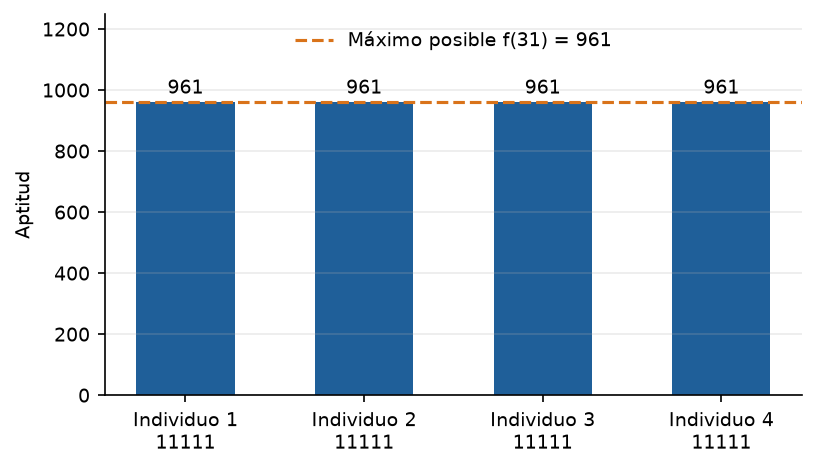
\includegraphics[width=0.85\textwidth]{p1_poblacion_final.png}
\caption{Población final y aptitud de cada individuo.}
\label{fig:p1-poblacion}
\end{figure}
\comoleerla
{una barra por individuo de la población final, con su cromosoma y su aptitud
sobre la barra.}
{los cuatro individuos son \PunoMejor{} con aptitud \PunoAptitud{}, y todas
las barras tocan la línea del máximo.}
{la población final ya no tiene diversidad: los cuatro individuos son
idénticos.}

\subsubsection{Pregunta de interpretación}
\label{sec:p1-interpretacion}

\textbf{¿Encontró el óptimo global?} Sí. El mejor cromosoma final es
\PunoMejor{}, con $x=\PunoX$ y aptitud \PunoAptitud{}. El máximo posible de
la función es $f(31)=\PunoOptimo$, así que coinciden. Lo encontró en la
generación \PunoPrimeraGen{}, después de \PunoGenAntes{} generaciones sin
mejorar (aptitud \PunoMeseta{}, que corresponde a $x=29$).

\textbf{Por qué veinte generaciones no garantizan hallarlo.}
\begin{itemize}
  \item \textbf{Población de solo cuatro individuos.} Con tan pocos
  individuos la variedad se agota rápido. En \PunoGenUniformes{} de las 20
  generaciones los cuatro individuos eran iguales, y cuando los padres son
  iguales el cruce no cambia nada.
  \item \textbf{Pérdida de diversidad.} \texttt{10010} se perdió en la primera
  generación, y con él el único cuarto bit en $1$. Desde ahí, ni la
  selección ni el cruce podían producir \texttt{11111}.
  \item \textbf{Estocasticidad de la mutación.} Solo la mutación podía
  recuperar ese bit. Si la población fuera toda \texttt{11101}, la
  probabilidad de que un descendiente se volviera \texttt{11111} sería
  $0{,}05\cdot0{,}95^4=\PunoProbHijo$ (\PunoProbHijoPorc{}), y la de que
  aparezca al menos uno entre los tres descendientes de una generación,
  \PunoProbGen{} (\PunoProbGenPorc{}). Con esa simplificación, la
  probabilidad de no verlo en 20 generaciones sería \PunoProbSinExito{}
  (\PunoProbSinExitoPorc{}). Es pequeña, pero no es cero.
  \item \textbf{Alcance del resultado.} Se ejecutó una sola semilla. El
  éxito observado no demuestra que el algoritmo lo halle siempre; solo
  muestra que, con esta semilla, la mutación llegó a tiempo.
\end{itemize}

%=====================================================================
\section{Punto 2. Ascenso de colinas y óptimos locales}

Se maximiza $f(x)$ sobre nueve estados, con vecinos $x-1$ y $x+1$ dentro del
dominio. El algoritmo elige el vecino de mayor valor y solo se mueve si hay
mejora estricta.

\subsection{Parte A: componente matemático y conceptual}

\noindent\textbf{1. Desde $x_0=0$.} Los vecinos de $0$ son solo el $1$, con
$f(1)=4>f(0)=1$, así que se mueve al $1$. En $1$ los vecinos son $0$ ($1$) y
$2$ ($7$); gana el $2$. En $2$ los vecinos son $1$ ($4$) y $3$ ($5$); el
mejor es $3$, pero $5<7$, así que no hay mejora y se detiene. Estados
visitados: $0,1,2$.

\noindent\textbf{2. Desde $x_0=4$.} En $4$ los vecinos son $3$ ($5$) y $5$
($6$); gana el $5$. En $5$ los vecinos son $4$ ($3$) y $6$ ($9$); gana el $6$.
En $6$ los vecinos son $5$ ($6$) y $7$ ($8$); el mejor es $8<9$, así que se
detiene. Estados visitados: $4,5,6$ (Tabla~\ref{tab:p2a-trazas}).

\begin{table}[H]
\centering
\small
\setlength{\tabcolsep}{6pt}
\renewcommand{\arraystretch}{1.15}
\begin{tabular}{|c|c|c|c|}
\hline
\rowcolor{encabezado}\textbf{Inicio $x_0$} & \textbf{Estados visitados} & \textbf{Estado final} & \textbf{$f$ final} \\
\hline
$0$ & $0$ $\to$ $1$ $\to$ $2$ & $2$ & $7$ \\
\hline
$4$ & $4$ $\to$ $5$ $\to$ $6$ & $6$ & $9$ \\
\hline
\end{tabular}
\caption{Ascenso de colinas calculado desde $x_0=0$ y desde $x_0=4$.}
\label{tab:p2a-trazas}
\end{table}


\noindent\textbf{3. Máximos locales y global.} Un máximo local es un estado
sin vecinos mejores. Hay dos: $x=2$ con $f=7$ y $x=6$ con $f=9$. El máximo
global es $x=6$, el de mayor valor de toda la función
(Tabla~\ref{tab:p2a-clasificacion}).

\begin{table}[H]
\centering
\small
\setlength{\tabcolsep}{6pt}
\renewcommand{\arraystretch}{1.15}
\begin{tabular}{|c|c|c|c|}
\hline
\rowcolor{encabezado}\textbf{$x$} & \textbf{$f(x)$} & \textbf{Vecinos} & \textbf{Clasificación} \\
\hline
$0$ & $1$ & $1$ & Ninguno \\
\hline
$1$ & $4$ & $0$, $2$ & Ninguno \\
\hline
$2$ & $7$ & $1$, $3$ & Máximo local \\
\hline
$3$ & $5$ & $2$, $4$ & Ninguno \\
\hline
$4$ & $3$ & $3$, $5$ & Ninguno \\
\hline
$5$ & $6$ & $4$, $6$ & Ninguno \\
\hline
$6$ & $9$ & $5$, $7$ & Máximo global \\
\hline
$7$ & $8$ & $6$, $8$ & Ninguno \\
\hline
$8$ & $5$ & $7$ & Ninguno \\
\hline
\end{tabular}
\caption{Clasificación de los nueve estados del espacio.}
\label{tab:p2a-clasificacion}
\end{table}


\noindent\textbf{4. Por qué importa el estado inicial.} El algoritmo es
determinista y voraz: siempre sube por la pendiente más cercana. Cada máximo
tiene su propia cuenca de atracción, es decir, el conjunto de inicios que
terminan en él. Los inicios $0$ a $3$ caen en el máximo local $2$ y los
inicios $4$ a $8$ en el global $6$. Empezar en una u otra cuenca cambia el
resultado.

\noindent\textbf{5. Estrategia y costo.} La estrategia es el reinicio
aleatorio: repetir el ascenso desde varios estados iniciales elegidos al azar
y conservar el mejor resultado. El costo es mayor número de evaluaciones de
la función, proporcional al número de reinicios. Además, no hay garantía de
éxito: todos los reinicios podrían caer en la cuenca del máximo local.

\subsection{Parte B: implementación en Python}

\subsubsection{Decisiones de implementación}

\begin{table}[H]
\centering\small
\renewcommand{\arraystretch}{1.15}
\begin{tabular}{|l|>{\raggedright\arraybackslash}p{9.6cm}|}
\hline
\textbf{Aspecto} & \textbf{Supuesto adoptado} \\ \hline
Aleatoriedad & Ninguna. El algoritmo es determinista y no usa generador. \\
\hline
Interfaz & \texttt{ascenso\_colinas(valores, inicio)} devuelve el estado
final y la lista de estados visitados, incluido el inicial. \\ \hline
Vecino elegido & El de mayor valor. Si hubiera un empate, \texttt{max}
devuelve el primero (el izquierdo); en estos datos no ocurre. \\ \hline
Parada & Se detiene cuando el mejor vecino no supera estrictamente el valor
actual. \\ \hline
Reinicios & Se calcula $1-(1-p)^k$ con $p$ igual a la proporción de inicios
que llegan al global, para $k=1,2,3,5$. \\ \hline
\end{tabular}
\caption{Decisiones de implementación del punto 2.}
\label{tab:p2-decisiones}
\end{table}

\subsubsection{Resultados}

\begin{table}[H]
\centering
\small
\setlength{\tabcolsep}{6pt}
\renewcommand{\arraystretch}{1.15}
\begin{tabular}{|c|c|c|c|c|}
\hline
\textbf{Estado inicial} & \textbf{Trayectoria} & \textbf{Estado final} & \textbf{Valor final} & \textbf{¿Global?} \\
\hline
$0$ & $0$ $\to$ $1$ $\to$ $2$ & $2$ & $7$ & No \\
\hline
$1$ & $1$ $\to$ $2$ & $2$ & $7$ & No \\
\hline
$2$ & $2$ & $2$ & $7$ & No \\
\hline
$3$ & $3$ $\to$ $2$ & $2$ & $7$ & No \\
\hline
$4$ & $4$ $\to$ $5$ $\to$ $6$ & $6$ & $9$ & Sí \\
\hline
$5$ & $5$ $\to$ $6$ & $6$ & $9$ & Sí \\
\hline
$6$ & $6$ & $6$ & $9$ & Sí \\
\hline
$7$ & $7$ $\to$ $6$ & $6$ & $9$ & Sí \\
\hline
$8$ & $8$ $\to$ $7$ $\to$ $6$ & $6$ & $9$ & Sí \\
\hline
\end{tabular}
\caption{Resultado del ascenso de colinas desde los nueve estados iniciales.}
\label{tab:p2b-trayectorias}
\end{table}

\comoleerla
{una fila por estado inicial, con su trayectoria, estado final, valor final
y si llegó al global.}
{los inicios $0$ a $3$ terminan en $2$ con valor $7$; los inicios $4$ a $8$
terminan en $6$ con valor $9$.}
{muestra las dos cuencas de atracción obtenidas al ejecutar la función.}

\begin{figure}[H]
\centering
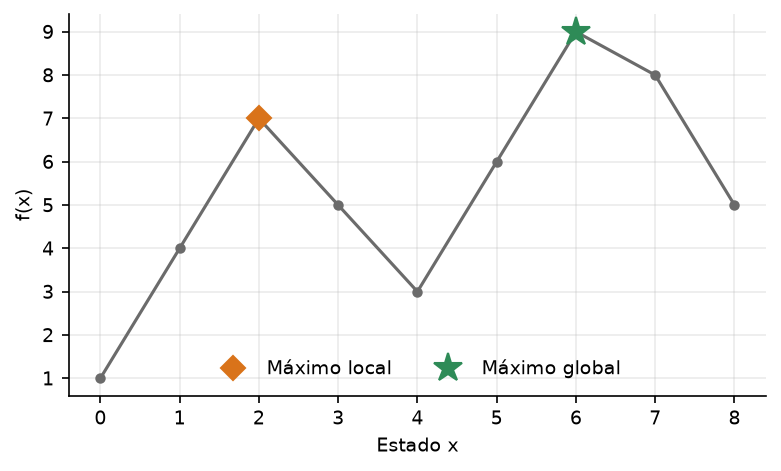
\includegraphics[width=0.85\textwidth]{p2_funcion.png}
\caption{Función $f(x)$ con los máximos local y global marcados.}
\label{fig:p2-funcion}
\end{figure}
\comoleerla
{estados en el eje horizontal y valor de la función en el vertical; el
rombo naranja es el máximo local y la estrella verde el global.}
{dos picos separados por un valle en $x=4$.}
{el valle impide que un ascenso que empieza a un lado alcance el pico del
otro lado.}

\begin{figure}[H]
\centering
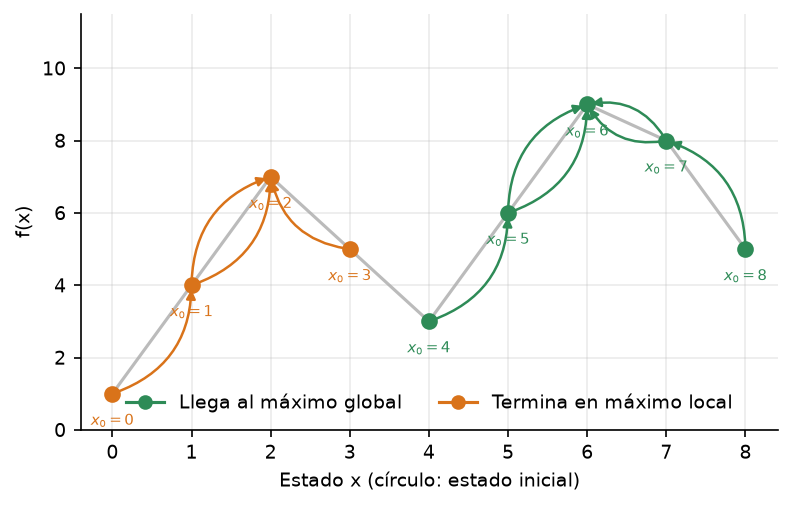
\includegraphics[width=0.85\textwidth]{p2_trayectorias.png}
\caption{Trayectorias del ascenso de colinas desde los nueve estados
iniciales.}
\label{fig:p2-trayectorias}
\end{figure}
\comoleerla
{cada flecha es un movimiento; el círculo marca el estado inicial y el color
indica el destino (verde: global, naranja: local).}
{los caminos que empiezan entre $0$ y $3$ suben al pico de $x=2$; los que
empiezan entre $4$ y $8$ suben al pico de $x=6$.}
{las flechas se curvan para que se distingan las trayectorias que comparten
tramos.}

\subsubsection{Pregunta de interpretación}

\textbf{Proporción que llega al máximo global.} \PdosExitos{} de los
\PdosTotal{} estados iniciales (\PdosProporcion{}) terminan en el global
$x=6$. Los demás terminan en el máximo local $x=2$.

\textbf{Relación con los reinicios aleatorios.}
\begin{itemize}
  \item Si el estado inicial se elige de forma uniforme, un solo intento
  llega al global con probabilidad \PdosFrac{}, igual a la proporción observada.
  \item Con $k$ reinicios independientes, la probabilidad de fallar en todos
  es $(\PdosFalloFrac)^k$, y la de al menos un éxito es $1-(\PdosFalloFrac)^k$
  (Tabla~\ref{tab:p2b-reinicios}).
\end{itemize}

\begin{table}[H]
\centering
\small
\setlength{\tabcolsep}{6pt}
\renewcommand{\arraystretch}{1.15}
\begin{tabular}{|c|c|}
\hline
\textbf{Reinicios $k$} & \textbf{$P(\text{al menos un éxito})$} \\
\hline
$1$ & $0{,}5556$ \\
\hline
$2$ & $0{,}8025$ \\
\hline
$3$ & $0{,}9122$ \\
\hline
$5$ & $0{,}9827$ \\
\hline
\end{tabular}
\caption{Probabilidad de alcanzar el máximo global con $k$ reinicios independientes desde un estado uniforme.}
\label{tab:p2b-reinicios}
\end{table}

\comoleerla
{una fila por número de reinicios $k$ con la probabilidad de al menos un
éxito.}
{pasa de \PdosProbUno{} con $k=1$ a \PdosProbTres{} con $k=3$ y a
\PdosProbCinco{} con $k=5$.}
{cada reinicio extra reduce por un factor \PdosFalloFrac{} la probabilidad de fallar,
pero nunca la lleva a cero: el éxito sigue sin estar garantizado.}

%=====================================================================
\section{Punto 3. Temple simulado: aceptación de soluciones peores}

Se minimiza $E(x)=x^2$ con $x\in\{-5,\dots,5\}$. Un movimiento con
$\Delta E\le0$ se acepta siempre. Uno con $\Delta E>0$ se acepta con
probabilidad $e^{-\Delta E/T}$, es decir, cuando $u<P$.

\subsection{Parte A: componente matemático y conceptual}

\noindent\textbf{1. Los tres casos.} Se usa $\Delta E=E(x_{nuevo})-E(x_{actual})$.
\begin{itemize}
  \item \textbf{Caso A} ($3\to2$, $T=5$, $u=0{,}70$): $\Delta E=4-9=-5$.
  Como $\Delta E\le0$, $P=1$ y se acepta, porque es una mejora.
  \item \textbf{Caso B} ($2\to3$, $T=5$, $u=0{,}30$): $\Delta E=9-4=5$ y
  $P=e^{-5/5}=e^{-1}\approx0{,}3679$. Como $0{,}30<0{,}3679$, se acepta
  aunque sea peor.
  \item \textbf{Caso C} ($2\to3$, $T=1$, $u=0{,}30$): $\Delta E=5$ y
  $P=e^{-5}\approx0{,}0067$. Como $0{,}30>0{,}0067$, se rechaza.
\end{itemize}

\begin{table}[H]
\centering
\small
\setlength{\tabcolsep}{6pt}
\renewcommand{\arraystretch}{1.15}
\begin{tabular}{|c|c|c|c|c|c|c|c|}
\hline
\rowcolor{encabezado}\textbf{Caso} & \textbf{Actual} & \textbf{Candidato} & \textbf{$T$} & \textbf{$u$} & \textbf{$\Delta E$} & \textbf{$P(\text{aceptar})$} & \textbf{Decisión} \\
\hline
A & $3$ & $2$ & $5$ & $0{,}70$ & $-5$ & $1{,}0000$ & Acepta \\
\hline
B & $2$ & $3$ & $5$ & $0{,}30$ & $5$ & $0{,}3679$ & Acepta \\
\hline
C & $2$ & $3$ & $1$ & $0{,}30$ & $5$ & $0{,}0067$ & Rechaza \\
\hline
\end{tabular}
\caption{Aceptación de cada transición analizada de forma independiente.}
\label{tab:p3a-casos}
\end{table}


\noindent\textbf{2. Influencia de la temperatura.} Los casos B y C tienen el
mismo $\Delta E$ y el mismo $u$, y solo cambia $T$. Con $T$ alta, la
probabilidad de aceptar un movimiento peor es grande (B). Con $T$ baja es
casi nula (C). Una temperatura alta favorece explorar; una baja, conservar
lo ya logrado.

\noindent\textbf{3. Enfriamiento demasiado rápido.} La temperatura baja antes
de que el algoritmo haya explorado. Entonces casi no acepta movimientos
peores y se comporta como un ascenso de colinas. Queda atrapado en el óptimo
local más cercano a su punto de partida.

\noindent\textbf{4. Comparación con ascenso de colinas.} El ascenso de
colinas mira a todos los vecinos, elige el mejor y solo se mueve si mejora.
El temple simulado evalúa un único vecino aleatorio y puede aceptarlo aunque
sea peor, con una probabilidad que depende de $T$. Esa posibilidad le permite
salir de óptimos locales.

\subsection{Parte B: implementación en Python}

\subsubsection{Decisiones de implementación}

\begin{table}[H]
\centering\small
\renewcommand{\arraystretch}{1.15}
\begin{tabular}{|l|>{\raggedright\arraybackslash}p{9.6cm}|}
\hline
\textbf{Aspecto} & \textbf{Supuesto adoptado} \\ \hline
Generador & \texttt{random.Random(42)}, creado una sola vez al inicio de
\texttt{temple\_simulado}. \\ \hline
Vecinos & Los válidos entre $x-1$ y $x+1$. En los extremos ($x=\pm5$) hay uno
solo y se elige ese, sin consumir llamadas aleatorias. \\ \hline
Orden por iteración & (1) \texttt{choice} del vecino, solo si hay dos;
(2) $u=$ \texttt{random()}, que se extrae siempre, incluso cuando
$\Delta E\le0$; (3) se acepta si $u<P$; (4) se actualiza la mejor solución
solo si mejora estrictamente. \\ \hline
Temperatura & La iteración $k$ usa $T_k=10\cdot0{,}90^{k-1}$; luego se enfría. \\
\hline
Historial & Por iteración: temperatura usada, candidato, $\Delta E$, $P$,
$u$, decisión, estado y energía actuales, mejor estado y mejor energía. Incluye
la fila 0 con el estado inicial ($x_0=5$, $E=25$, que también es la mejor
solución hasta ese momento) y 100 filas más de iteraciones. La fila 0 no cuenta
como iteración ni decide nada. \\ \hline
\end{tabular}
\caption{Decisiones de implementación del punto 3.}
\label{tab:p3-decisiones}
\end{table}

\subsubsection{Resultados}

\begin{table}[H]
\centering
\small
\setlength{\tabcolsep}{6pt}
\renewcommand{\arraystretch}{1.15}
\begin{tabular}{|c|c|c|c|c|}
\hline
\rowcolor{encabezado}\textbf{Estado inicial} & \textbf{Mejor solución} & \textbf{Energía mínima} & \textbf{Estado final} & \textbf{Energía final} \\
\hline
$5$ & $0$ & $0$ & $0$ & $0$ \\
\hline
\end{tabular}
\caption{Resultado del temple simulado tras 100 iteraciones.}
\label{tab:p3b-resumen}
\end{table}

\comoleerla
{una fila con el estado inicial, la mejor solución, la energía mínima y el
estado y la energía finales.}
{la mejor solución es $x=\PtresMejor$ con energía mínima \PtresEnergia{}. El
estado final también es $x=\PtresFinal$.}
{en esta ejecución el estado final coincide con la mejor solución; el
historial muestra que no siempre fue así durante el recorrido.}

\begin{table}[H]
\centering
\scriptsize
\setlength{\tabcolsep}{3pt}
\renewcommand{\arraystretch}{1.15}
\begin{tabular}{|c|c|c|c|c|c|c|c|c|c|}
\hline
\rowcolor{encabezado}\textbf{Iter.} & \textbf{$T$} & \textbf{Iter.} & \textbf{$T$} & \textbf{Iter.} & \textbf{$T$} & \textbf{Iter.} & \textbf{$T$} & \textbf{Iter.} & \textbf{$T$} \\
\hline
\cellcolor{iteracion}{\bfseries\boldmath $1$} & $10{,}0000$ & \cellcolor{iteracion}{\bfseries\boldmath $21$} & $1{,}2158$ & \cellcolor{iteracion}{\bfseries\boldmath $41$} & $0{,}1478$ & \cellcolor{iteracion}{\bfseries\boldmath $61$} & $0{,}0180$ & \cellcolor{iteracion}{\bfseries\boldmath $81$} & $0{,}0022$ \\
\hline
\cellcolor{iteracion}{\bfseries\boldmath $2$} & \cellcolor{cebra}$9{,}0000$ & \cellcolor{iteracion}{\bfseries\boldmath $22$} & \cellcolor{cebra}$1{,}0942$ & \cellcolor{iteracion}{\bfseries\boldmath $42$} & \cellcolor{cebra}$0{,}1330$ & \cellcolor{iteracion}{\bfseries\boldmath $62$} & \cellcolor{cebra}$0{,}0162$ & \cellcolor{iteracion}{\bfseries\boldmath $82$} & \cellcolor{cebra}$0{,}0020$ \\
\hline
\cellcolor{iteracion}{\bfseries\boldmath $3$} & $8{,}1000$ & \cellcolor{iteracion}{\bfseries\boldmath $23$} & $0{,}9848$ & \cellcolor{iteracion}{\bfseries\boldmath $43$} & $0{,}1197$ & \cellcolor{iteracion}{\bfseries\boldmath $63$} & $0{,}0146$ & \cellcolor{iteracion}{\bfseries\boldmath $83$} & $0{,}0018$ \\
\hline
\cellcolor{iteracion}{\bfseries\boldmath $4$} & \cellcolor{cebra}$7{,}2900$ & \cellcolor{iteracion}{\bfseries\boldmath $24$} & \cellcolor{cebra}$0{,}8863$ & \cellcolor{iteracion}{\bfseries\boldmath $44$} & \cellcolor{cebra}$0{,}1078$ & \cellcolor{iteracion}{\bfseries\boldmath $64$} & \cellcolor{cebra}$0{,}0131$ & \cellcolor{iteracion}{\bfseries\boldmath $84$} & \cellcolor{cebra}$0{,}0016$ \\
\hline
\cellcolor{destacado}{\bfseries\boldmath $5$} & \cellcolor{destacado}$6{,}5610$ & \cellcolor{iteracion}{\bfseries\boldmath $25$} & $0{,}7977$ & \cellcolor{iteracion}{\bfseries\boldmath $45$} & $0{,}0970$ & \cellcolor{iteracion}{\bfseries\boldmath $65$} & $0{,}0118$ & \cellcolor{iteracion}{\bfseries\boldmath $85$} & $0{,}0014$ \\
\hline
\cellcolor{destacado}{\bfseries\boldmath $6$} & \cellcolor{destacado}$5{,}9049$ & \cellcolor{iteracion}{\bfseries\boldmath $26$} & \cellcolor{cebra}$0{,}7179$ & \cellcolor{iteracion}{\bfseries\boldmath $46$} & \cellcolor{cebra}$0{,}0873$ & \cellcolor{iteracion}{\bfseries\boldmath $66$} & \cellcolor{cebra}$0{,}0106$ & \cellcolor{iteracion}{\bfseries\boldmath $86$} & \cellcolor{cebra}$0{,}0013$ \\
\hline
\cellcolor{destacado}{\bfseries\boldmath $7$} & \cellcolor{destacado}$5{,}3144$ & \cellcolor{iteracion}{\bfseries\boldmath $27$} & $0{,}6461$ & \cellcolor{iteracion}{\bfseries\boldmath $47$} & $0{,}0786$ & \cellcolor{iteracion}{\bfseries\boldmath $67$} & $0{,}0096$ & \cellcolor{iteracion}{\bfseries\boldmath $87$} & $0{,}0012$ \\
\hline
\cellcolor{iteracion}{\bfseries\boldmath $8$} & \cellcolor{cebra}$4{,}7830$ & \cellcolor{destacado}{\bfseries\boldmath $28$} & \cellcolor{destacado}$0{,}5815$ & \cellcolor{iteracion}{\bfseries\boldmath $48$} & \cellcolor{cebra}$0{,}0707$ & \cellcolor{iteracion}{\bfseries\boldmath $68$} & \cellcolor{cebra}$0{,}0086$ & \cellcolor{iteracion}{\bfseries\boldmath $88$} & \cellcolor{cebra}$0{,}0010$ \\
\hline
\cellcolor{iteracion}{\bfseries\boldmath $9$} & $4{,}3047$ & \cellcolor{iteracion}{\bfseries\boldmath $29$} & $0{,}5233$ & \cellcolor{iteracion}{\bfseries\boldmath $49$} & $0{,}0636$ & \cellcolor{iteracion}{\bfseries\boldmath $69$} & $0{,}0077$ & \cellcolor{iteracion}{\bfseries\boldmath $89$} & $0{,}0009$ \\
\hline
\cellcolor{iteracion}{\bfseries\boldmath $10$} & \cellcolor{cebra}$3{,}8742$ & \cellcolor{iteracion}{\bfseries\boldmath $30$} & \cellcolor{cebra}$0{,}4710$ & \cellcolor{iteracion}{\bfseries\boldmath $50$} & \cellcolor{cebra}$0{,}0573$ & \cellcolor{iteracion}{\bfseries\boldmath $70$} & \cellcolor{cebra}$0{,}0070$ & \cellcolor{iteracion}{\bfseries\boldmath $90$} & \cellcolor{cebra}$0{,}0008$ \\
\hline
\cellcolor{iteracion}{\bfseries\boldmath $11$} & $3{,}4868$ & \cellcolor{iteracion}{\bfseries\boldmath $31$} & $0{,}4239$ & \cellcolor{iteracion}{\bfseries\boldmath $51$} & $0{,}0515$ & \cellcolor{iteracion}{\bfseries\boldmath $71$} & $0{,}0063$ & \cellcolor{iteracion}{\bfseries\boldmath $91$} & $0{,}0008$ \\
\hline
\cellcolor{destacado}{\bfseries\boldmath $12$} & \cellcolor{destacado}$3{,}1381$ & \cellcolor{iteracion}{\bfseries\boldmath $32$} & \cellcolor{cebra}$0{,}3815$ & \cellcolor{iteracion}{\bfseries\boldmath $52$} & \cellcolor{cebra}$0{,}0464$ & \cellcolor{iteracion}{\bfseries\boldmath $72$} & \cellcolor{cebra}$0{,}0056$ & \cellcolor{iteracion}{\bfseries\boldmath $92$} & \cellcolor{cebra}$0{,}0007$ \\
\hline
\cellcolor{iteracion}{\bfseries\boldmath $13$} & $2{,}8243$ & \cellcolor{iteracion}{\bfseries\boldmath $33$} & $0{,}3434$ & \cellcolor{iteracion}{\bfseries\boldmath $53$} & $0{,}0417$ & \cellcolor{iteracion}{\bfseries\boldmath $73$} & $0{,}0051$ & \cellcolor{iteracion}{\bfseries\boldmath $93$} & $0{,}0006$ \\
\hline
\cellcolor{iteracion}{\bfseries\boldmath $14$} & \cellcolor{cebra}$2{,}5419$ & \cellcolor{iteracion}{\bfseries\boldmath $34$} & \cellcolor{cebra}$0{,}3090$ & \cellcolor{iteracion}{\bfseries\boldmath $54$} & \cellcolor{cebra}$0{,}0376$ & \cellcolor{iteracion}{\bfseries\boldmath $74$} & \cellcolor{cebra}$0{,}0046$ & \cellcolor{iteracion}{\bfseries\boldmath $94$} & \cellcolor{cebra}$0{,}0006$ \\
\hline
\cellcolor{destacado}{\bfseries\boldmath $15$} & \cellcolor{destacado}$2{,}2877$ & \cellcolor{iteracion}{\bfseries\boldmath $35$} & $0{,}2781$ & \cellcolor{iteracion}{\bfseries\boldmath $55$} & $0{,}0338$ & \cellcolor{iteracion}{\bfseries\boldmath $75$} & $0{,}0041$ & \cellcolor{iteracion}{\bfseries\boldmath $95$} & $0{,}0005$ \\
\hline
\cellcolor{destacado}{\bfseries\boldmath $16$} & \cellcolor{destacado}$2{,}0589$ & \cellcolor{iteracion}{\bfseries\boldmath $36$} & \cellcolor{cebra}$0{,}2503$ & \cellcolor{iteracion}{\bfseries\boldmath $56$} & \cellcolor{cebra}$0{,}0304$ & \cellcolor{iteracion}{\bfseries\boldmath $76$} & \cellcolor{cebra}$0{,}0037$ & \cellcolor{iteracion}{\bfseries\boldmath $96$} & \cellcolor{cebra}$0{,}0004$ \\
\hline
\cellcolor{iteracion}{\bfseries\boldmath $17$} & $1{,}8530$ & \cellcolor{iteracion}{\bfseries\boldmath $37$} & $0{,}2253$ & \cellcolor{iteracion}{\bfseries\boldmath $57$} & $0{,}0274$ & \cellcolor{iteracion}{\bfseries\boldmath $77$} & $0{,}0033$ & \cellcolor{iteracion}{\bfseries\boldmath $97$} & $0{,}0004$ \\
\hline
\cellcolor{iteracion}{\bfseries\boldmath $18$} & \cellcolor{cebra}$1{,}6677$ & \cellcolor{iteracion}{\bfseries\boldmath $38$} & \cellcolor{cebra}$0{,}2028$ & \cellcolor{iteracion}{\bfseries\boldmath $58$} & \cellcolor{cebra}$0{,}0247$ & \cellcolor{iteracion}{\bfseries\boldmath $78$} & \cellcolor{cebra}$0{,}0030$ & \cellcolor{iteracion}{\bfseries\boldmath $98$} & \cellcolor{cebra}$0{,}0004$ \\
\hline
\cellcolor{iteracion}{\bfseries\boldmath $19$} & $1{,}5009$ & \cellcolor{iteracion}{\bfseries\boldmath $39$} & $0{,}1825$ & \cellcolor{iteracion}{\bfseries\boldmath $59$} & $0{,}0222$ & \cellcolor{iteracion}{\bfseries\boldmath $79$} & $0{,}0027$ & \cellcolor{iteracion}{\bfseries\boldmath $99$} & $0{,}0003$ \\
\hline
\cellcolor{destacado}{\bfseries\boldmath $20$} & \cellcolor{destacado}$1{,}3509$ & \cellcolor{iteracion}{\bfseries\boldmath $40$} & \cellcolor{cebra}$0{,}1642$ & \cellcolor{iteracion}{\bfseries\boldmath $60$} & \cellcolor{cebra}$0{,}0200$ & \cellcolor{iteracion}{\bfseries\boldmath $80$} & \cellcolor{cebra}$0{,}0024$ & \cellcolor{iteracion}{\bfseries\boldmath $100$} & \cellcolor{cebra}$0{,}0003$ \\
\hline
\end{tabular}
\caption{Historial de la temperatura usada en cada iteración. En la tabla, el fondo azul marca la columna de iteración; el gris claro alterna las filas; el fondo amarillo, con el número en negrita, señala la iteración 5 (se alcanza la mejor energía) y las iteraciones 6, 7, 12, 15, 16, 20, 28 (se aceptó un candidato peor).}
\label{tab:p3b-temperatura}
\end{table}

\comoleerla
{cinco bloques de columnas con la iteración y la temperatura usada en ella.}
{la temperatura baja de \PtresTempInicial{} en la iteración $1$ a
\PtresTempFinal{} en la iteración $100$.}
{cada paso multiplica por $0{,}90$, así que la caída es geométrica.}

\begin{table}[H]
\centering
\scriptsize
\setlength{\tabcolsep}{1.2pt}
\renewcommand{\arraystretch}{1.15}
\begin{tabular}{|c|c|c|c|c|c|c|c|c|c|c|c|c|c|c|}
\hline
\rowcolor{encabezado}\textbf{Iter.} & \textbf{$x$ actual} & \textbf{$E$ actual} & \textbf{$x$ mejor} & \textbf{$E$ mejor} & \textbf{Iter.} & \textbf{$x$ actual} & \textbf{$E$ actual} & \textbf{$x$ mejor} & \textbf{$E$ mejor} & \textbf{Iter.} & \textbf{$x$ actual} & \textbf{$E$ actual} & \textbf{$x$ mejor} & \textbf{$E$ mejor} \\
\hline
\cellcolor{destacado}{\bfseries\boldmath $0$} & \cellcolor{destacado}$5$ & \cellcolor{destacado}$25$ & \cellcolor{destacado}$5$ & \cellcolor{destacado}$25$ & \cellcolor{iteracion}{\bfseries\boldmath $34$} & $0$ & $0$ & $0$ & $0$ & \cellcolor{iteracion}{\bfseries\boldmath $68$} & $0$ & $0$ & $0$ & $0$ \\
\hline
\cellcolor{iteracion}{\bfseries\boldmath $1$} & \cellcolor{cebra}$4$ & \cellcolor{cebra}$16$ & \cellcolor{cebra}$4$ & \cellcolor{cebra}$16$ & \cellcolor{iteracion}{\bfseries\boldmath $35$} & \cellcolor{cebra}$0$ & \cellcolor{cebra}$0$ & \cellcolor{cebra}$0$ & \cellcolor{cebra}$0$ & \cellcolor{iteracion}{\bfseries\boldmath $69$} & \cellcolor{cebra}$0$ & \cellcolor{cebra}$0$ & \cellcolor{cebra}$0$ & \cellcolor{cebra}$0$ \\
\hline
\cellcolor{iteracion}{\bfseries\boldmath $2$} & $3$ & $9$ & $3$ & $9$ & \cellcolor{iteracion}{\bfseries\boldmath $36$} & $0$ & $0$ & $0$ & $0$ & \cellcolor{iteracion}{\bfseries\boldmath $70$} & $0$ & $0$ & $0$ & $0$ \\
\hline
\cellcolor{iteracion}{\bfseries\boldmath $3$} & \cellcolor{cebra}$2$ & \cellcolor{cebra}$4$ & \cellcolor{cebra}$2$ & \cellcolor{cebra}$4$ & \cellcolor{iteracion}{\bfseries\boldmath $37$} & \cellcolor{cebra}$0$ & \cellcolor{cebra}$0$ & \cellcolor{cebra}$0$ & \cellcolor{cebra}$0$ & \cellcolor{iteracion}{\bfseries\boldmath $71$} & \cellcolor{cebra}$0$ & \cellcolor{cebra}$0$ & \cellcolor{cebra}$0$ & \cellcolor{cebra}$0$ \\
\hline
\cellcolor{iteracion}{\bfseries\boldmath $4$} & $1$ & $1$ & $1$ & $1$ & \cellcolor{iteracion}{\bfseries\boldmath $38$} & $0$ & $0$ & $0$ & $0$ & \cellcolor{iteracion}{\bfseries\boldmath $72$} & $0$ & $0$ & $0$ & $0$ \\
\hline
\cellcolor{destacado}{\bfseries\boldmath $5$} & \cellcolor{destacado}$0$ & \cellcolor{destacado}$0$ & \cellcolor{destacado}$0$ & \cellcolor{destacado}$0$ & \cellcolor{iteracion}{\bfseries\boldmath $39$} & \cellcolor{cebra}$0$ & \cellcolor{cebra}$0$ & \cellcolor{cebra}$0$ & \cellcolor{cebra}$0$ & \cellcolor{iteracion}{\bfseries\boldmath $73$} & \cellcolor{cebra}$0$ & \cellcolor{cebra}$0$ & \cellcolor{cebra}$0$ & \cellcolor{cebra}$0$ \\
\hline
\cellcolor{destacado}{\bfseries\boldmath $6$} & \cellcolor{destacado}$-1$ & \cellcolor{destacado}$1$ & \cellcolor{destacado}$0$ & \cellcolor{destacado}$0$ & \cellcolor{iteracion}{\bfseries\boldmath $40$} & $0$ & $0$ & $0$ & $0$ & \cellcolor{iteracion}{\bfseries\boldmath $74$} & $0$ & $0$ & $0$ & $0$ \\
\hline
\cellcolor{destacado}{\bfseries\boldmath $7$} & \cellcolor{destacado}$-2$ & \cellcolor{destacado}$4$ & \cellcolor{destacado}$0$ & \cellcolor{destacado}$0$ & \cellcolor{iteracion}{\bfseries\boldmath $41$} & \cellcolor{cebra}$0$ & \cellcolor{cebra}$0$ & \cellcolor{cebra}$0$ & \cellcolor{cebra}$0$ & \cellcolor{iteracion}{\bfseries\boldmath $75$} & \cellcolor{cebra}$0$ & \cellcolor{cebra}$0$ & \cellcolor{cebra}$0$ & \cellcolor{cebra}$0$ \\
\hline
\cellcolor{iteracion}{\bfseries\boldmath $8$} & $-2$ & $4$ & $0$ & $0$ & \cellcolor{iteracion}{\bfseries\boldmath $42$} & $0$ & $0$ & $0$ & $0$ & \cellcolor{iteracion}{\bfseries\boldmath $76$} & $0$ & $0$ & $0$ & $0$ \\
\hline
\cellcolor{iteracion}{\bfseries\boldmath $9$} & \cellcolor{cebra}$-1$ & \cellcolor{cebra}$1$ & \cellcolor{cebra}$0$ & \cellcolor{cebra}$0$ & \cellcolor{iteracion}{\bfseries\boldmath $43$} & \cellcolor{cebra}$0$ & \cellcolor{cebra}$0$ & \cellcolor{cebra}$0$ & \cellcolor{cebra}$0$ & \cellcolor{iteracion}{\bfseries\boldmath $77$} & \cellcolor{cebra}$0$ & \cellcolor{cebra}$0$ & \cellcolor{cebra}$0$ & \cellcolor{cebra}$0$ \\
\hline
\cellcolor{iteracion}{\bfseries\boldmath $10$} & $0$ & $0$ & $0$ & $0$ & \cellcolor{iteracion}{\bfseries\boldmath $44$} & $0$ & $0$ & $0$ & $0$ & \cellcolor{iteracion}{\bfseries\boldmath $78$} & $0$ & $0$ & $0$ & $0$ \\
\hline
\cellcolor{iteracion}{\bfseries\boldmath $11$} & \cellcolor{cebra}$0$ & \cellcolor{cebra}$0$ & \cellcolor{cebra}$0$ & \cellcolor{cebra}$0$ & \cellcolor{iteracion}{\bfseries\boldmath $45$} & \cellcolor{cebra}$0$ & \cellcolor{cebra}$0$ & \cellcolor{cebra}$0$ & \cellcolor{cebra}$0$ & \cellcolor{iteracion}{\bfseries\boldmath $79$} & \cellcolor{cebra}$0$ & \cellcolor{cebra}$0$ & \cellcolor{cebra}$0$ & \cellcolor{cebra}$0$ \\
\hline
\cellcolor{destacado}{\bfseries\boldmath $12$} & \cellcolor{destacado}$-1$ & \cellcolor{destacado}$1$ & \cellcolor{destacado}$0$ & \cellcolor{destacado}$0$ & \cellcolor{iteracion}{\bfseries\boldmath $46$} & $0$ & $0$ & $0$ & $0$ & \cellcolor{iteracion}{\bfseries\boldmath $80$} & $0$ & $0$ & $0$ & $0$ \\
\hline
\cellcolor{iteracion}{\bfseries\boldmath $13$} & \cellcolor{cebra}$0$ & \cellcolor{cebra}$0$ & \cellcolor{cebra}$0$ & \cellcolor{cebra}$0$ & \cellcolor{iteracion}{\bfseries\boldmath $47$} & \cellcolor{cebra}$0$ & \cellcolor{cebra}$0$ & \cellcolor{cebra}$0$ & \cellcolor{cebra}$0$ & \cellcolor{iteracion}{\bfseries\boldmath $81$} & \cellcolor{cebra}$0$ & \cellcolor{cebra}$0$ & \cellcolor{cebra}$0$ & \cellcolor{cebra}$0$ \\
\hline
\cellcolor{iteracion}{\bfseries\boldmath $14$} & $0$ & $0$ & $0$ & $0$ & \cellcolor{iteracion}{\bfseries\boldmath $48$} & $0$ & $0$ & $0$ & $0$ & \cellcolor{iteracion}{\bfseries\boldmath $82$} & $0$ & $0$ & $0$ & $0$ \\
\hline
\cellcolor{destacado}{\bfseries\boldmath $15$} & \cellcolor{destacado}$1$ & \cellcolor{destacado}$1$ & \cellcolor{destacado}$0$ & \cellcolor{destacado}$0$ & \cellcolor{iteracion}{\bfseries\boldmath $49$} & \cellcolor{cebra}$0$ & \cellcolor{cebra}$0$ & \cellcolor{cebra}$0$ & \cellcolor{cebra}$0$ & \cellcolor{iteracion}{\bfseries\boldmath $83$} & \cellcolor{cebra}$0$ & \cellcolor{cebra}$0$ & \cellcolor{cebra}$0$ & \cellcolor{cebra}$0$ \\
\hline
\cellcolor{destacado}{\bfseries\boldmath $16$} & \cellcolor{destacado}$2$ & \cellcolor{destacado}$4$ & \cellcolor{destacado}$0$ & \cellcolor{destacado}$0$ & \cellcolor{iteracion}{\bfseries\boldmath $50$} & $0$ & $0$ & $0$ & $0$ & \cellcolor{iteracion}{\bfseries\boldmath $84$} & $0$ & $0$ & $0$ & $0$ \\
\hline
\cellcolor{iteracion}{\bfseries\boldmath $17$} & \cellcolor{cebra}$2$ & \cellcolor{cebra}$4$ & \cellcolor{cebra}$0$ & \cellcolor{cebra}$0$ & \cellcolor{iteracion}{\bfseries\boldmath $51$} & \cellcolor{cebra}$0$ & \cellcolor{cebra}$0$ & \cellcolor{cebra}$0$ & \cellcolor{cebra}$0$ & \cellcolor{iteracion}{\bfseries\boldmath $85$} & \cellcolor{cebra}$0$ & \cellcolor{cebra}$0$ & \cellcolor{cebra}$0$ & \cellcolor{cebra}$0$ \\
\hline
\cellcolor{iteracion}{\bfseries\boldmath $18$} & $1$ & $1$ & $0$ & $0$ & \cellcolor{iteracion}{\bfseries\boldmath $52$} & $0$ & $0$ & $0$ & $0$ & \cellcolor{iteracion}{\bfseries\boldmath $86$} & $0$ & $0$ & $0$ & $0$ \\
\hline
\cellcolor{iteracion}{\bfseries\boldmath $19$} & \cellcolor{cebra}$0$ & \cellcolor{cebra}$0$ & \cellcolor{cebra}$0$ & \cellcolor{cebra}$0$ & \cellcolor{iteracion}{\bfseries\boldmath $53$} & \cellcolor{cebra}$0$ & \cellcolor{cebra}$0$ & \cellcolor{cebra}$0$ & \cellcolor{cebra}$0$ & \cellcolor{iteracion}{\bfseries\boldmath $87$} & \cellcolor{cebra}$0$ & \cellcolor{cebra}$0$ & \cellcolor{cebra}$0$ & \cellcolor{cebra}$0$ \\
\hline
\cellcolor{destacado}{\bfseries\boldmath $20$} & \cellcolor{destacado}$1$ & \cellcolor{destacado}$1$ & \cellcolor{destacado}$0$ & \cellcolor{destacado}$0$ & \cellcolor{iteracion}{\bfseries\boldmath $54$} & $0$ & $0$ & $0$ & $0$ & \cellcolor{iteracion}{\bfseries\boldmath $88$} & $0$ & $0$ & $0$ & $0$ \\
\hline
\cellcolor{iteracion}{\bfseries\boldmath $21$} & \cellcolor{cebra}$1$ & \cellcolor{cebra}$1$ & \cellcolor{cebra}$0$ & \cellcolor{cebra}$0$ & \cellcolor{iteracion}{\bfseries\boldmath $55$} & \cellcolor{cebra}$0$ & \cellcolor{cebra}$0$ & \cellcolor{cebra}$0$ & \cellcolor{cebra}$0$ & \cellcolor{iteracion}{\bfseries\boldmath $89$} & \cellcolor{cebra}$0$ & \cellcolor{cebra}$0$ & \cellcolor{cebra}$0$ & \cellcolor{cebra}$0$ \\
\hline
\cellcolor{iteracion}{\bfseries\boldmath $22$} & $1$ & $1$ & $0$ & $0$ & \cellcolor{iteracion}{\bfseries\boldmath $56$} & $0$ & $0$ & $0$ & $0$ & \cellcolor{iteracion}{\bfseries\boldmath $90$} & $0$ & $0$ & $0$ & $0$ \\
\hline
\cellcolor{iteracion}{\bfseries\boldmath $23$} & \cellcolor{cebra}$0$ & \cellcolor{cebra}$0$ & \cellcolor{cebra}$0$ & \cellcolor{cebra}$0$ & \cellcolor{iteracion}{\bfseries\boldmath $57$} & \cellcolor{cebra}$0$ & \cellcolor{cebra}$0$ & \cellcolor{cebra}$0$ & \cellcolor{cebra}$0$ & \cellcolor{iteracion}{\bfseries\boldmath $91$} & \cellcolor{cebra}$0$ & \cellcolor{cebra}$0$ & \cellcolor{cebra}$0$ & \cellcolor{cebra}$0$ \\
\hline
\cellcolor{iteracion}{\bfseries\boldmath $24$} & $0$ & $0$ & $0$ & $0$ & \cellcolor{iteracion}{\bfseries\boldmath $58$} & $0$ & $0$ & $0$ & $0$ & \cellcolor{iteracion}{\bfseries\boldmath $92$} & $0$ & $0$ & $0$ & $0$ \\
\hline
\cellcolor{iteracion}{\bfseries\boldmath $25$} & \cellcolor{cebra}$0$ & \cellcolor{cebra}$0$ & \cellcolor{cebra}$0$ & \cellcolor{cebra}$0$ & \cellcolor{iteracion}{\bfseries\boldmath $59$} & \cellcolor{cebra}$0$ & \cellcolor{cebra}$0$ & \cellcolor{cebra}$0$ & \cellcolor{cebra}$0$ & \cellcolor{iteracion}{\bfseries\boldmath $93$} & \cellcolor{cebra}$0$ & \cellcolor{cebra}$0$ & \cellcolor{cebra}$0$ & \cellcolor{cebra}$0$ \\
\hline
\cellcolor{iteracion}{\bfseries\boldmath $26$} & $0$ & $0$ & $0$ & $0$ & \cellcolor{iteracion}{\bfseries\boldmath $60$} & $0$ & $0$ & $0$ & $0$ & \cellcolor{iteracion}{\bfseries\boldmath $94$} & $0$ & $0$ & $0$ & $0$ \\
\hline
\cellcolor{iteracion}{\bfseries\boldmath $27$} & \cellcolor{cebra}$0$ & \cellcolor{cebra}$0$ & \cellcolor{cebra}$0$ & \cellcolor{cebra}$0$ & \cellcolor{iteracion}{\bfseries\boldmath $61$} & \cellcolor{cebra}$0$ & \cellcolor{cebra}$0$ & \cellcolor{cebra}$0$ & \cellcolor{cebra}$0$ & \cellcolor{iteracion}{\bfseries\boldmath $95$} & \cellcolor{cebra}$0$ & \cellcolor{cebra}$0$ & \cellcolor{cebra}$0$ & \cellcolor{cebra}$0$ \\
\hline
\cellcolor{destacado}{\bfseries\boldmath $28$} & \cellcolor{destacado}$1$ & \cellcolor{destacado}$1$ & \cellcolor{destacado}$0$ & \cellcolor{destacado}$0$ & \cellcolor{iteracion}{\bfseries\boldmath $62$} & $0$ & $0$ & $0$ & $0$ & \cellcolor{iteracion}{\bfseries\boldmath $96$} & $0$ & $0$ & $0$ & $0$ \\
\hline
\cellcolor{iteracion}{\bfseries\boldmath $29$} & \cellcolor{cebra}$1$ & \cellcolor{cebra}$1$ & \cellcolor{cebra}$0$ & \cellcolor{cebra}$0$ & \cellcolor{iteracion}{\bfseries\boldmath $63$} & \cellcolor{cebra}$0$ & \cellcolor{cebra}$0$ & \cellcolor{cebra}$0$ & \cellcolor{cebra}$0$ & \cellcolor{iteracion}{\bfseries\boldmath $97$} & \cellcolor{cebra}$0$ & \cellcolor{cebra}$0$ & \cellcolor{cebra}$0$ & \cellcolor{cebra}$0$ \\
\hline
\cellcolor{iteracion}{\bfseries\boldmath $30$} & $1$ & $1$ & $0$ & $0$ & \cellcolor{iteracion}{\bfseries\boldmath $64$} & $0$ & $0$ & $0$ & $0$ & \cellcolor{iteracion}{\bfseries\boldmath $98$} & $0$ & $0$ & $0$ & $0$ \\
\hline
\cellcolor{iteracion}{\bfseries\boldmath $31$} & \cellcolor{cebra}$0$ & \cellcolor{cebra}$0$ & \cellcolor{cebra}$0$ & \cellcolor{cebra}$0$ & \cellcolor{iteracion}{\bfseries\boldmath $65$} & \cellcolor{cebra}$0$ & \cellcolor{cebra}$0$ & \cellcolor{cebra}$0$ & \cellcolor{cebra}$0$ & \cellcolor{iteracion}{\bfseries\boldmath $99$} & \cellcolor{cebra}$0$ & \cellcolor{cebra}$0$ & \cellcolor{cebra}$0$ & \cellcolor{cebra}$0$ \\
\hline
\cellcolor{iteracion}{\bfseries\boldmath $32$} & $0$ & $0$ & $0$ & $0$ & \cellcolor{iteracion}{\bfseries\boldmath $66$} & $0$ & $0$ & $0$ & $0$ & \cellcolor{iteracion}{\bfseries\boldmath $100$} & $0$ & $0$ & $0$ & $0$ \\
\hline
\cellcolor{iteracion}{\bfseries\boldmath $33$} & \cellcolor{cebra}$0$ & \cellcolor{cebra}$0$ & \cellcolor{cebra}$0$ & \cellcolor{cebra}$0$ & \cellcolor{iteracion}{\bfseries\boldmath $67$} & \cellcolor{cebra}$0$ & \cellcolor{cebra}$0$ & \cellcolor{cebra}$0$ & \cellcolor{cebra}$0$ & \cellcolor{cebra} & \cellcolor{cebra} & \cellcolor{cebra} & \cellcolor{cebra} & \cellcolor{cebra} \\
\hline
\end{tabular}
\caption{Historial del estado actual y de la mejor solución con sus energías (la iteración 0 es el estado inicial). En la tabla, el fondo azul marca la columna de iteración; el gris claro alterna las filas; el fondo amarillo, con el número en negrita, señala la iteración 0 (estado inicial, $x=5$ y $E=25$), la iteración 5 (se alcanza la mejor energía) y las iteraciones 6, 7, 12, 15, 16, 20, 28 (se aceptó un candidato peor).}
\label{tab:p3b-energia}
\end{table}

\comoleerla
{tres bloques con la iteración, el estado actual y su energía, y la mejor
solución y su energía. La iteración 0 es el estado inicial.}
{la energía parte de \PtresEnergiaInicial{} en $x_0=5$ (iteración 0), llega a $0$ en la
iteración \PtresIterMejor{} y vuelve a subir a \PtresEnergiaSalida{} en la
iteración \PtresIterSalida{}.}
{la mejor energía no sube nunca; la actual sí puede subir cuando se acepta un
movimiento peor.}

\begin{figure}[H]
\centering
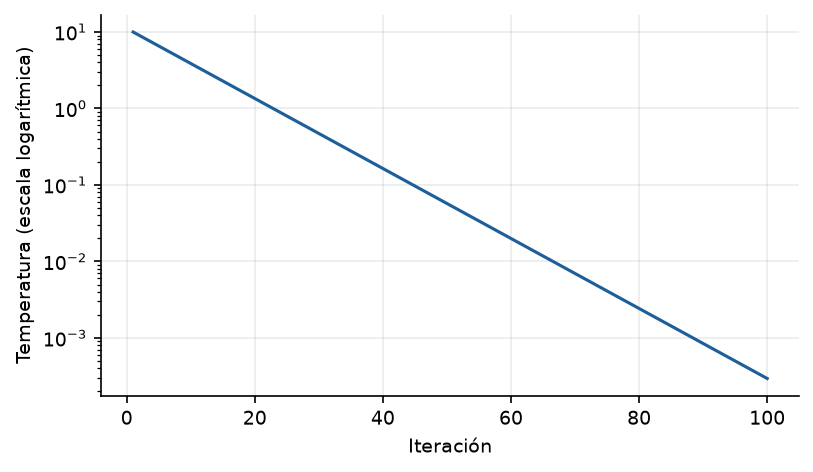
\includegraphics[width=0.85\textwidth]{p3_temperatura.png}
\caption{Temperatura por iteración en escala logarítmica.}
\label{fig:p3-temperatura}
\end{figure}
\comoleerla
{iteraciones en el eje horizontal y temperatura en el vertical, en escala
logarítmica.}
{una recta descendente.}
{una caída geométrica es una recta en escala logarítmica, con pendiente
$\ln0{,}90$.}

\begin{figure}[H]
\centering
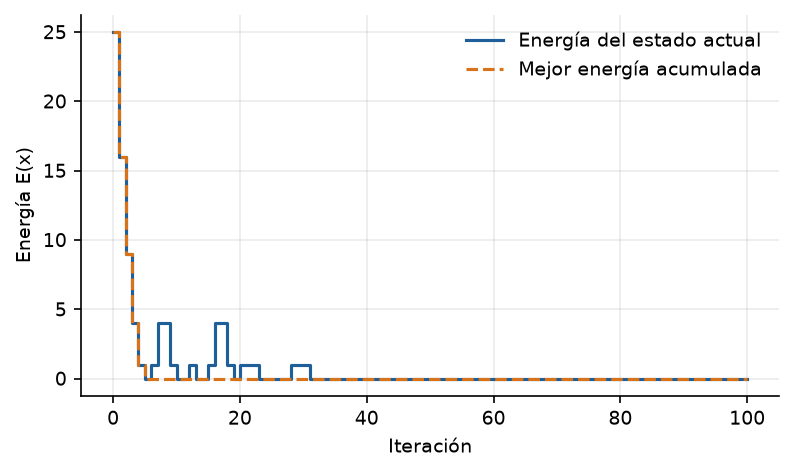
\includegraphics[width=0.85\textwidth]{p3_energia.png}
\caption{Energía del estado actual y mejor energía acumulada por
iteración.}
\label{fig:p3-energia}
\end{figure}
\comoleerla
{dos escalones desde la iteración 0 (estado inicial, $E=25$): la energía del
estado actual (azul) y la mejor energía vista hasta ese momento (naranja
punteada).}
{el estado actual desciende hasta $0$ en la iteración \PtresIterMejor{}, vuelve
a subir hasta energía \PtresEnergiaMaxima{} en varias ocasiones y desde la
iteración \PtresDesdeFijo{} queda fijo en $0$. La mejor energía
llega a $0$ y se queda.}
{al principio la temperatura alta permite subir; al final, con $T$ baja, el
estado ya no se mueve de $0$.}

\subsubsection{Pregunta de interpretación}

\textbf{¿Por qué guardar la mejor solución además del estado actual?}
\begin{itemize}
  \item El temple simulado puede aceptar movimientos peores, así que el
  estado actual puede alejarse de lo mejor que ha visto.
  \item En esta ejecución el estado final coincide con la mejor solución
  ($x=\PtresMejor$), pero eso fue una coincidencia del recorrido, no una
  garantía del método.
  \item El historial lo prueba: la mejor energía \PtresEnergia{} se alcanzó
  en la iteración \PtresIterMejor{}, y en la iteración \PtresIterSalida{} el
  estado actual ya había subido a energía \PtresEnergiaSalida{}. En
  \PtresPeorQueMejor{} de las 100 iteraciones el estado actual fue peor que
  la mejor solución. Si el algoritmo se hubiera detenido en cualquiera de
  ellas, devolver solo el estado actual habría entregado una solución peor
  que una ya encontrada.
  \item Se aceptaron \PtresPeores{} de \PtresPropuestasPeores{} candidatos
  peores, el último en la iteración \PtresUltimoPeor{} (con
  $T=\PtresTempUltimoPeor$). En la segunda mitad (iteraciones $51$ a $100$)
  hubo \PtresPropuestasSegunda{} propuestas peores y ninguna se aceptó,
  porque $T$ ya era muy baja. Mientras $T$ es alta, el riesgo de alejarse de lo mejor
  existe, y guardar la mejor solución lo cubre.
\end{itemize}

%=====================================================================
\section{Punto 4. ACO: elección de rutas y actualización de feromonas}

Una hormiga en el nodo $A$ elige su siguiente nodo con
$p_{Aj}=\tau_{Aj}^{\alpha}\eta_{Aj}^{\beta}/\sum_k\tau_{Ak}^{\alpha}
\eta_{Ak}^{\beta}$, con $\eta_{Aj}=1/d_{Aj}$, $\alpha=1$ y $\beta=2$.

\subsection{Parte A: componente matemático y conceptual}

\noindent\textbf{1. Pesos y probabilidades.} El peso de cada arista es
$\tau\eta^2$. Para $A\to B$ es $1\cdot(1/2)^2=0{,}25$; para $A\to C$,
$2\cdot(1/4)^2=0{,}125$; para $A\to D$, $1\cdot(1/5)^2=0{,}04$. La suma de
los pesos es \PcuatroSumaPesos{}. La probabilidad de cada arista es su peso
dividido entre esa suma (Tabla~\ref{tab:p4a-pesos}).

\begin{table}[H]
\centering
\small
\setlength{\tabcolsep}{6pt}
\renewcommand{\arraystretch}{1.15}
\begin{tabular}{|c|c|c|c|c|}
\hline
\rowcolor{encabezado}\textbf{Arista} & \textbf{$d$} & \textbf{$\tau$} & \textbf{Peso $\tau\eta^2$} & \textbf{Probabilidad} \\
\hline
$A\to B$ & $2$ & $1$ & $0{,}2500$ & $0{,}6024$ \\
\hline
$A\to C$ & $4$ & $2$ & $0{,}1250$ & $0{,}3012$ \\
\hline
$A\to D$ & $5$ & $1$ & $0{,}0400$ & $0{,}0964$ \\
\hline
Suma &  &  & $0{,}4150$ & $1{,}0000$ \\
\hline
\end{tabular}
\caption{Peso y probabilidad de elección desde el nodo $A$.}
\label{tab:p4a-pesos}
\end{table}


\noindent\textbf{2. Alternativa más probable.} Es $A\to B$, con
\PcuatroProbAPorc{}. Su elección no está garantizada: la regla es
probabilística, así que la hormiga puede ir a $C$ o a $D$ con las
probabilidades restantes.

\noindent\textbf{3. Actualización de feromonas.} Con $\rho=0{,}2$, $Q=10$ y
$L=10$, el depósito en $A\to B$ es $\Delta\tau_{AB}=Q/L=1$. Las otras dos
aristas no reciben depósito. Primero se evapora el 20\,\% y luego se suma
el depósito: $\tau_{AB}=0{,}8\cdot1+1=1{,}8$, $\tau_{AC}=0{,}8\cdot2=1{,}6$
y $\tau_{AD}=0{,}8\cdot1=0{,}8$ (Tabla~\ref{tab:p4a-feromonas}).

\begin{table}[H]
\centering
\small
\setlength{\tabcolsep}{6pt}
\renewcommand{\arraystretch}{1.15}
\begin{tabular}{|c|c|c|c|c|}
\hline
\textbf{Arista} & \textbf{$\tau$ actual} & \textbf{$(1-\rho)\tau$} & \textbf{$\Delta\tau$} & \textbf{$\tau$ nueva} \\
\hline
$A\to B$ & $1{,}0$ & $0{,}8$ & $1{,}0$ & $1{,}8$ \\
\hline
$A\to C$ & $2{,}0$ & $1{,}6$ & $0{,}0$ & $1{,}6$ \\
\hline
$A\to D$ & $1{,}0$ & $0{,}8$ & $0{,}0$ & $0{,}8$ \\
\hline
\end{tabular}
\caption{Actualización de la feromona tras una hormiga con $L=10$ que usa $A\to B$.}
\label{tab:p4a-feromonas}
\end{table}


\noindent\textbf{4. Evaporación y dominio de la feromona.}
\begin{itemize}
  \item \textbf{Función de la evaporación.} Hace que la feromona de rutas
  que dejan de usarse se desvanezca. Así el sistema olvida rutas antiguas y
  evita convergir de forma prematura a una sola.
  \item \textbf{Si la feromona domina.} El término $\tau^\alpha$ pesa más
  que la información heurística $\eta^\beta$. Entonces las hormigas siguen la
  ruta con más feromona aunque no sea la mejor. El sistema se estanca y se
  pierde la exploración de rutas alternativas.
\end{itemize}

\subsection{Parte B: implementación en Python}

\subsubsection{Decisiones de implementación}

\begin{table}[H]
\centering\small
\renewcommand{\arraystretch}{1.15}
\begin{tabular}{|l|>{\raggedright\arraybackslash}p{9.6cm}|}
\hline
\textbf{Aspecto} & \textbf{Supuesto adoptado} \\ \hline
Generador & \texttt{numpy.random.default\_rng(42)}, creado una sola vez al
inicio de \texttt{aco}. \\ \hline
Elección de las hormigas & Una sola llamada por iteración:
\texttt{rng.choice(3, size=10, p=p)}. Las diez hormigas eligen de forma
independiente con las mismas probabilidades. \\ \hline
Orden por iteración & (1) probabilidades con las feromonas actuales;
(2) elección de las diez hormigas; (3) evaporación de todas las rutas,
$\tau\leftarrow0{,}8\,\tau$; (4) cada hormiga suma $Q/L_r$ a la ruta que
eligió. \\ \hline
Registro & Las probabilidades guardadas son las usadas para elegir en esa
iteración. Las feromonas guardadas son las del final de la iteración. \\
\hline
Mejor ruta observada & La de menor longitud entre las rutas elegidas al
menos una vez. \\ \hline
\end{tabular}
\caption{Decisiones de implementación del punto 4.}
\label{tab:p4-decisiones}
\end{table}

\subsubsection{Resultados}

\begin{table}[H]
\centering
\small
\setlength{\tabcolsep}{6pt}
\renewcommand{\arraystretch}{1.15}
\begin{tabular}{|c|c|c|c|}
\hline
\rowcolor{encabezado}\textbf{Ruta} & \textbf{Longitud} & \textbf{Frecuencia} & \textbf{Proporción} \\
\hline
A-B-Z & $6$ & $185$ & $92{,}5$\,\% \\
\hline
A-C-Z & $8$ & $10$ & $5{,}0$\,\% \\
\hline
A-D-Z & $10$ & $5$ & $2{,}5$\,\% \\
\hline
Total &  & $200$ & $100{,}0$\,\% \\
\hline
\end{tabular}
\caption{Frecuencia total de elección de cada ruta en las 200 decisiones.}
\label{tab:p4b-frecuencias}
\end{table}

\comoleerla
{una fila por ruta con su longitud, cuántas veces fue elegida y qué parte de
las \PcuatroDecisiones{} decisiones representa.}
{$A$-$B$-$Z$ fue elegida \PcuatroBFrec{} veces (\PcuatroBPorc{}),
$A$-$C$-$Z$ \PcuatroCFrec{} veces (\PcuatroCPorc{}) y $A$-$D$-$Z$
\PcuatroDFrec{} veces (\PcuatroDPorc{}).}
{la ruta más corta concentra casi todas las elecciones.}

\begin{table}[H]
\centering
\small
\setlength{\tabcolsep}{6pt}
\renewcommand{\arraystretch}{1.15}
\begin{tabular}{|c|c|c|c|}
\hline
\textbf{Ruta} & \textbf{Feromona inicial} & \textbf{Feromona final} & \textbf{Probabilidad final} \\
\hline
A-B-Z & $1$ & $81{,}9229$ & $0{,}9979$ \\
\hline
A-C-Z & $1$ & $0{,}2356$ & $0{,}0016$ \\
\hline
A-D-Z & $1$ & $0{,}1090$ & $0{,}0005$ \\
\hline
\end{tabular}
\caption{Feromona de cada ruta al terminar la iteración 20 y probabilidad de elección que implicaría.}
\label{tab:p4b-feromonas}
\end{table}

\comoleerla
{una fila por ruta con la feromona inicial, la final y la probabilidad de
elección que esa feromona implica.}
{la feromona de $A$-$B$-$Z$ es \PcuatroBFer{}, frente a \PcuatroCFer{} y
\PcuatroDFer{} en las otras dos.}
{la ruta elegida recibe depósito en cada iteración y las otras solo se
evaporan.}

\begin{table}[H]
\centering
\small
\setlength{\tabcolsep}{6pt}
\renewcommand{\arraystretch}{1.15}
\begin{tabular}{|c|c|c|c|c|c|c|c|}
\hline
\textbf{Iter.} & \textbf{A-B-Z} & \textbf{A-C-Z} & \textbf{A-D-Z} & \textbf{Iter.} & \textbf{A-B-Z} & \textbf{A-C-Z} & \textbf{A-D-Z} \\
\hline
$1$ & $4$ & $4$ & $2$ & $11$ & $10$ & $0$ & $0$ \\
\hline
$2$ & $6$ & $3$ & $1$ & $12$ & $10$ & $0$ & $0$ \\
\hline
$3$ & $6$ & $3$ & $1$ & $13$ & $10$ & $0$ & $0$ \\
\hline
$4$ & $9$ & $0$ & $1$ & $14$ & $10$ & $0$ & $0$ \\
\hline
$5$ & $10$ & $0$ & $0$ & $15$ & $10$ & $0$ & $0$ \\
\hline
$6$ & $10$ & $0$ & $0$ & $16$ & $10$ & $0$ & $0$ \\
\hline
$7$ & $10$ & $0$ & $0$ & $17$ & $10$ & $0$ & $0$ \\
\hline
$8$ & $10$ & $0$ & $0$ & $18$ & $10$ & $0$ & $0$ \\
\hline
$9$ & $10$ & $0$ & $0$ & $19$ & $10$ & $0$ & $0$ \\
\hline
$10$ & $10$ & $0$ & $0$ & $20$ & $10$ & $0$ & $0$ \\
\hline
\end{tabular}
\caption{Elecciones de cada ruta por iteración (diez hormigas).}
\label{tab:p4b-conteo}
\end{table}

\comoleerla
{dos bloques de columnas con la iteración y cuántas de las diez hormigas
eligieron cada ruta.}
{en la iteración $1$ eligen \PcuatroPrimeraB{}, \PcuatroPrimeraC{} y
\PcuatroPrimeraD{} hormigas; desde la iteración \PcuatroIterTodas{} las diez
eligen $A$-$B$-$Z$.}
{es el momento en que la preferencia pasa de repartida a total.}

\begin{table}[H]
\centering
\small
\setlength{\tabcolsep}{6pt}
\renewcommand{\arraystretch}{1.15}
\begin{tabular}{|c|c|c|c|c|c|c|c|}
\hline
\rowcolor{encabezado}\textbf{Iter.} & \textbf{A-B-Z} & \textbf{A-C-Z} & \textbf{A-D-Z} & \textbf{Iter.} & \textbf{A-B-Z} & \textbf{A-C-Z} & \textbf{A-D-Z} \\
\hline
\cellcolor{destacado}{\bfseries\boldmath $1$} & \cellcolor{destacado}$0{,}5202$ & \cellcolor{destacado}$0{,}2926$ & \cellcolor{destacado}$0{,}1873$ & \cellcolor{iteracion}{\bfseries\boldmath $11$} & $0{,}9777$ & $0{,}0172$ & $0{,}0051$ \\
\hline
\cellcolor{iteracion}{\bfseries\boldmath $2$} & \cellcolor{cebra}$0{,}6362$ & \cellcolor{cebra}$0{,}2780$ & \cellcolor{cebra}$0{,}0859$ & \cellcolor{iteracion}{\bfseries\boldmath $12$} & \cellcolor{cebra}$0{,}9827$ & \cellcolor{cebra}$0{,}0133$ & \cellcolor{cebra}$0{,}0039$ \\
\hline
\cellcolor{iteracion}{\bfseries\boldmath $3$} & $0{,}7307$ & $0{,}2159$ & $0{,}0534$ & \cellcolor{iteracion}{\bfseries\boldmath $13$} & $0{,}9865$ & $0{,}0104$ & $0{,}0031$ \\
\hline
\cellcolor{iteracion}{\bfseries\boldmath $4$} & \cellcolor{cebra}$0{,}7604$ & \cellcolor{cebra}$0{,}1964$ & \cellcolor{cebra}$0{,}0432$ & \cellcolor{iteracion}{\bfseries\boldmath $14$} & \cellcolor{cebra}$0{,}9894$ & \cellcolor{cebra}$0{,}0082$ & \cellcolor{cebra}$0{,}0024$ \\
\hline
\cellcolor{iteracion}{\bfseries\boldmath $5$} & $0{,}8448$ & $0{,}1197$ & $0{,}0355$ & \cellcolor{iteracion}{\bfseries\boldmath $15$} & $0{,}9917$ & $0{,}0064$ & $0{,}0019$ \\
\hline
\cellcolor{iteracion}{\bfseries\boldmath $6$} & \cellcolor{cebra}$0{,}8986$ & \cellcolor{cebra}$0{,}0783$ & \cellcolor{cebra}$0{,}0232$ & \cellcolor{iteracion}{\bfseries\boldmath $16$} & \cellcolor{cebra}$0{,}9934$ & \cellcolor{cebra}$0{,}0051$ & \cellcolor{cebra}$0{,}0015$ \\
\hline
\cellcolor{iteracion}{\bfseries\boldmath $7$} & $0{,}9292$ & $0{,}0546$ & $0{,}0162$ & \cellcolor{iteracion}{\bfseries\boldmath $17$} & $0{,}9948$ & $0{,}0040$ & $0{,}0012$ \\
\hline
\cellcolor{iteracion}{\bfseries\boldmath $8$} & \cellcolor{cebra}$0{,}9486$ & \cellcolor{cebra}$0{,}0396$ & \cellcolor{cebra}$0{,}0117$ & \cellcolor{iteracion}{\bfseries\boldmath $18$} & \cellcolor{cebra}$0{,}9959$ & \cellcolor{cebra}$0{,}0032$ & \cellcolor{cebra}$0{,}0009$ \\
\hline
\cellcolor{iteracion}{\bfseries\boldmath $9$} & $0{,}9617$ & $0{,}0295$ & $0{,}0087$ & \cellcolor{iteracion}{\bfseries\boldmath $19$} & $0{,}9967$ & $0{,}0025$ & $0{,}0008$ \\
\hline
\cellcolor{iteracion}{\bfseries\boldmath $10$} & \cellcolor{cebra}$0{,}9710$ & \cellcolor{cebra}$0{,}0224$ & \cellcolor{cebra}$0{,}0066$ & \cellcolor{iteracion}{\bfseries\boldmath $20$} & \cellcolor{cebra}$0{,}9974$ & \cellcolor{cebra}$0{,}0020$ & \cellcolor{cebra}$0{,}0006$ \\
\hline
\end{tabular}
\caption{Probabilidad de elección de cada ruta al inicio de cada iteración. En la tabla, el fondo azul marca la columna de iteración; el gris claro alterna las filas; el fondo amarillo, con el número en negrita, señala la iteración 1, primera desde la cual A-B-Z es la ruta más probable en todas las iteraciones siguientes.}
\label{tab:p4b-probabilidades}
\end{table}

\comoleerla
{dos bloques con la iteración y la probabilidad de cada ruta al inicio de
ella.}
{la probabilidad de $A$-$B$-$Z$ sube de \PcuatroBIni{} a \PcuatroBFin{} y las
de las otras dos bajan a \PcuatroCFin{} y \PcuatroDFin{}.}
{la feromona acumulada se suma a la información heurística y cambia las
probabilidades iteración a iteración.}

\begin{figure}[H]
\centering
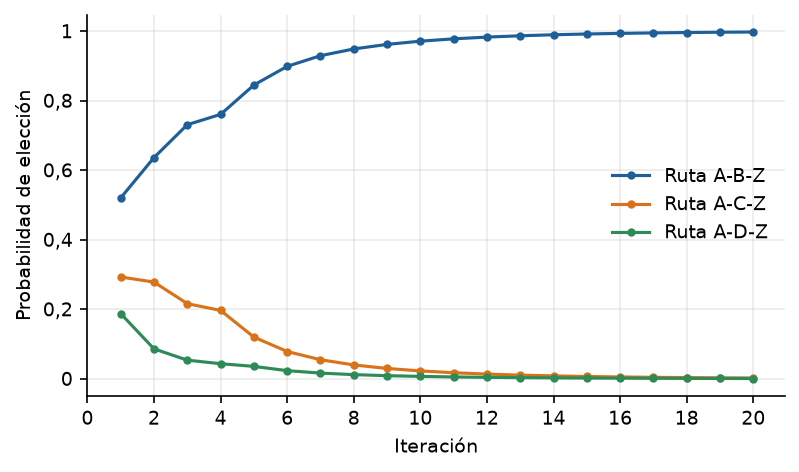
\includegraphics[width=0.85\textwidth]{p4_probabilidades.png}
\caption{Probabilidad de elección de cada ruta por iteración.}
\label{fig:p4-probabilidades}
\end{figure}
\comoleerla
{una línea por ruta; el eje vertical es la probabilidad con que cada hormiga
elige esa ruta en esa iteración.}
{la línea de $A$-$B$-$Z$ sube y se acerca a $1$; las otras dos bajan hacia
$0$.}
{es el efecto de la feromona acumulada sobre la preferencia heurística
inicial.}

\begin{figure}[H]
\centering
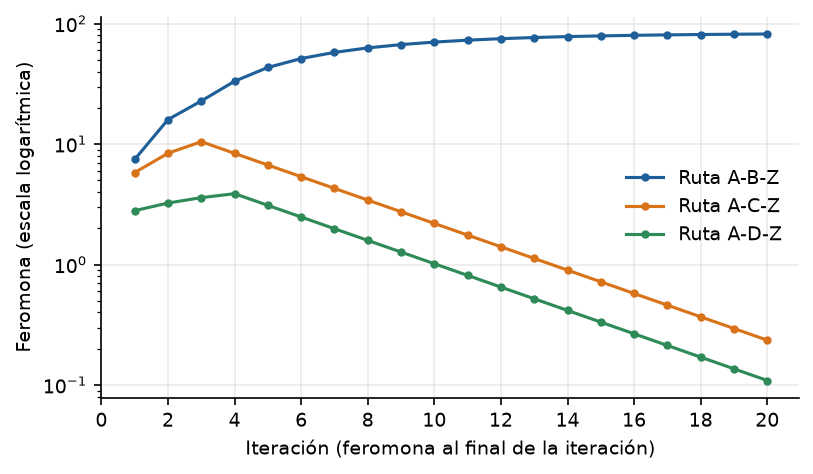
\includegraphics[width=0.85\textwidth]{p4_feromonas.png}
\caption{Feromona de cada ruta por iteración en escala logarítmica.}
\label{fig:p4-feromonas}
\end{figure}
\comoleerla
{una línea por ruta; el eje vertical, logarítmico, es la feromona al final de
cada iteración.}
{la de $A$-$B$-$Z$ crece y se estabiliza cerca de \PcuatroBFer{}. La de
$A$-$C$-$Z$ sube hasta la iteración \PcuatroIterPicoC{} (llega a
\PcuatroPicoC{}) y la de $A$-$D$-$Z$ hasta la \PcuatroIterPicoD{}; después
ambas caen en línea recta.}
{sin depósito, la evaporación multiplica por $0{,}8$ en cada iteración, lo
que en escala logarítmica es una recta.}

\begin{figure}[H]
\centering
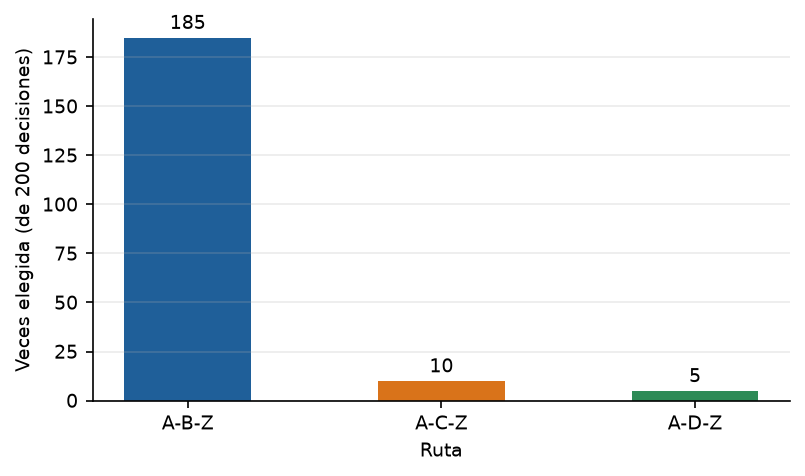
\includegraphics[width=0.85\textwidth]{p4_frecuencias.png}
\caption{Frecuencia total de elección de cada ruta.}
\label{fig:p4-frecuencias}
\end{figure}
\comoleerla
{una barra por ruta con las veces que fue elegida sobre las 200 decisiones.}
{la barra de $A$-$B$-$Z$ domina y las otras dos son muy bajas.}
{es el resumen de la Tabla~\ref{tab:p4b-frecuencias} en forma gráfica.}

\subsubsection{Pregunta de interpretación}

\textbf{Mejor ruta observada.} Es $A$-$B$-$Z$, de longitud $6$. Además es la
más elegida (\PcuatroBFrec{} de \PcuatroDecisiones{} decisiones).

\textbf{Cómo influyen la calidad de las rutas y la experiencia colectiva.}
\begin{itemize}
  \item \textbf{Calidad de la ruta, parte heurística.} Con las feromonas
  iguales en la iteración $1$, solo cuenta $\eta^\beta$: las probabilidades
  son \PcuatroBIni{}, \PcuatroCIni{} y \PcuatroDIni{}. La ruta corta ya parte
  con ventaja.
  \item \textbf{Calidad de la ruta, parte del depósito.} Cada hormiga
  deposita $Q/L_r$: \PcuatroBDep{} en $A$-$B$-$Z$, \PcuatroCDep{} en
  $A$-$C$-$Z$ y \PcuatroDDep{} en $A$-$D$-$Z$. Una ruta corta deja más
  feromona por cada hormiga que la usa.
  \item \textbf{Experiencia colectiva.} Lo que dejaron las hormigas de una
  iteración cambia las probabilidades de la siguiente. La de $A$-$B$-$Z$
  pasa de \PcuatroBIni{} a \PcuatroBDos{} en la iteración $2$, a
  \PcuatroBCinco{} en la iteración $5$ y a \PcuatroBFin{} en la $20$.
  \item \textbf{Refuerzo y olvido.} La ruta preferida recibe más depósito,
  lo que la hace aún más probable. Las otras solo se evaporan. $A$-$C$-$Z$
  se eligió por última vez en la iteración \PcuatroUltimaC{} y $A$-$D$-$Z$ en
  la iteración \PcuatroUltimaD{}.
  \item \textbf{Costo de la convergencia rápida.} Desde la iteración
  \PcuatroIterTodas{} no se explora ninguna otra ruta. Aquí la ruta
  reforzada es además la más corta, pero el mecanismo no distingue: si una
  ruta peor hubiera recibido más depósito al inicio, la habría reforzado igual.
\end{itemize}

%=====================================================================
\section{Punto 5. PSO: movimiento de partículas y memoria}

Se minimiza una función con partículas que se mueven con
$v_{nuevo}=wv+c_1r_1(p_{best}-x)+c_2r_2(g_{best}-x)$ y
$x_{nuevo}=x+v_{nuevo}$, con $w=0{,}5$ y $c_1=c_2=1{,}5$.

\subsection{Parte A: componente matemático y conceptual}

\noindent\textbf{1 y 2. Términos, velocidad, posición y aptitud.} La
partícula tiene $x=4$, $v=-1$, $p_{best}=2$ y $g_{best}=1$, con
$r_1=0{,}4$ y $r_2=0{,}6$. Los tres términos y el resultado están en la
Tabla~\ref{tab:p5a-terminos}. La partícula pasa de $x=4$ a $x=-0{,}4$, con
$f(-0{,}4)=0{,}16$.

\begin{table}[H]
\centering
\small
\setlength{\tabcolsep}{6pt}
\renewcommand{\arraystretch}{1.15}
\begin{tabular}{|l|l|c|}
\hline
\rowcolor{encabezado}\textbf{Concepto} & \textbf{Expresión} & \textbf{Valor} \\
\hline
Inercia & $w\,v=0{,}5\cdot(-1)$ & $-0{,}50$ \\
\hline
Cognitivo & $c_1r_1(p_{best}-x)=1{,}5\cdot0{,}4\cdot(2-4)$ & $-1{,}20$ \\
\hline
Social & $c_2r_2(g_{best}-x)=1{,}5\cdot0{,}6\cdot(1-4)$ & $-2{,}70$ \\
\hline
Nueva velocidad & inercia + cognitivo + social & $-4{,}40$ \\
\hline
Nueva posición & $x+v_{nuevo}=4+(-4{,}4)$ & $-0{,}40$ \\
\hline
Aptitud & $f(-0{,}4)$ & $0{,}16$ \\
\hline
\end{tabular}
\caption{Cálculo de un paso de la partícula con $r_1=0{,}4$ y $r_2=0{,}6$.}
\label{tab:p5a-terminos}
\end{table}


\noindent\textbf{3. Actualización de memorias.} Se compara la nueva aptitud
con la de cada memoria (Tabla~\ref{tab:p5a-memorias}). Como $0{,}16<4=
f(p_{best})$, se actualiza $p_{best}=-0{,}4$. Como $0{,}16<1=f(g_{best})$ y
las demás partículas no han mejorado, también se actualiza $g_{best}=-0{,}4$.

\begin{table}[H]
\centering
\small
\setlength{\tabcolsep}{6pt}
\renewcommand{\arraystretch}{1.15}
\begin{tabular}{|c|c|c|c|}
\hline
\textbf{Memoria} & \textbf{Aptitud actual} & \textbf{Aptitud nueva} & \textbf{¿Se actualiza?} \\
\hline
$p_{best}$ & $4{,}00$ & $0{,}16$ & Sí \\
\hline
$g_{best}$ & $1{,}00$ & $0{,}16$ & Sí \\
\hline
\end{tabular}
\caption{Actualización de las memorias personal y global.}
\label{tab:p5a-memorias}
\end{table}


\noindent\textbf{4. Mejor posición personal y global.} La mejor posición
personal es la memoria individual de cada partícula: el mejor punto por el que
ella misma ha pasado. La mejor posición global es la mejor de todo el
enjambre, y es la misma para todas las partículas.

\noindent\textbf{5. Intercambio de información en PSO y en ACO.}
\begin{itemize}
  \item \textbf{En PSO} la información viaja de forma directa: $g_{best}$ es
  una posición que todas las partículas leen en cada iteración.
  \item \textbf{En ACO} la información es indirecta: las hormigas depositan
  feromona en el entorno y otras la leen después. Además, esa feromona se
  evapora, así que la información se desvanece con el tiempo. En PSO,
  $g_{best}$ se conserva hasta que aparece algo mejor.
\end{itemize}

\subsection{Parte B: implementación en Python}

\subsubsection{Decisiones de implementación}

\begin{table}[H]
\centering\small
\renewcommand{\arraystretch}{1.15}
\begin{tabular}{|l|>{\raggedright\arraybackslash}p{9.6cm}|}
\hline
\textbf{Aspecto} & \textbf{Supuesto adoptado} \\ \hline
Generador & \texttt{numpy.random.default\_rng(42)}, creado una sola vez al
inicio de \texttt{pso}. \\ \hline
Orden de llamadas & Primero las posiciones iniciales:
\texttt{rng.uniform(-5, 5, size=(10, 2))}. En cada iteración, \texttt{r1} y
luego \texttt{r2}, cada una con \texttt{rng.uniform(0, 1, size=(10, 2))}. Así
$r_1$ y $r_2$ son independientes por partícula, dimensión e iteración. \\
\hline
Memorias iniciales & $p_{best}$ igual a la posición inicial de cada
partícula. $g_{best}$ igual a la mejor posición inicial. \\ \hline
Actualización & Todas las partículas usan el mismo $g_{best}$ de la
iteración. Después se evalúa y se actualizan primero las memorias personales
y luego la global, solo con mejora estricta. \\ \hline
Límites & Una coordenada fuera de $[-5,5]$ se ajusta al límite y su
componente de velocidad se pone en cero. \\ \hline
Historial & Mejor aptitud global en la iteración 0 (inicial) y tras cada una
de las 30 iteraciones: 31 valores. \\ \hline
\end{tabular}
\caption{Decisiones de implementación del punto 5.}
\label{tab:p5-decisiones}
\end{table}

\subsubsection{Resultados}

\begin{table}[H]
\centering
\small
\setlength{\tabcolsep}{6pt}
\renewcommand{\arraystretch}{1.15}
\begin{tabular}{|c|c|c|}
\hline
\rowcolor{encabezado}\textbf{Mejor posición $(x,y)$} & \textbf{$f(x,y)$} & \textbf{Distancia al origen} \\
\hline
$(-1{,}848\times10^{-4},\;1{,}388\times10^{-5})$ & $3{,}434\times10^{-8}$ & $1{,}853\times10^{-4}$ \\
\hline
\end{tabular}
\caption{Mejor posición global tras 30 iteraciones.}
\label{tab:p5b-resumen}
\end{table}

\comoleerla
{una fila con la mejor posición global, su valor de la función y su distancia
al origen.}
{la mejor posición es $(\PcincoX,\;\PcincoY)$, con $f=\PcincoF$ y distancia
\PcincoDist{} al origen.}
{está muy cerca de $(0,0)$ pero no es exactamente $(0,0)$.}

\begin{table}[H]
\centering
\footnotesize
\setlength{\tabcolsep}{4pt}
\renewcommand{\arraystretch}{1.15}
\begin{tabular}{|c|c|c|c|c|c|}
\hline
\rowcolor{encabezado}\textbf{Iter.} & \textbf{Mejor aptitud global} & \textbf{Iter.} & \textbf{Mejor aptitud global} & \textbf{Iter.} & \textbf{Mejor aptitud global} \\
\hline
\cellcolor{destacado}{\bfseries\boldmath $0$} & \cellcolor{destacado}$7{,}760\times10^{0}$ & \cellcolor{iteracion}{\bfseries\boldmath $11$} & $1{,}024\times10^{-2}$ & \cellcolor{iteracion}{\bfseries\boldmath $22$} & $8{,}881\times10^{-6}$ \\
\hline
\cellcolor{iteracion}{\bfseries\boldmath $1$} & \cellcolor{cebra}$6{,}533\times10^{-1}$ & \cellcolor{iteracion}{\bfseries\boldmath $12$} & \cellcolor{cebra}$1{,}819\times10^{-3}$ & \cellcolor{iteracion}{\bfseries\boldmath $23$} & \cellcolor{cebra}$5{,}834\times10^{-6}$ \\
\hline
\cellcolor{iteracion}{\bfseries\boldmath $2$} & $5{,}698\times10^{-1}$ & \cellcolor{iteracion}{\bfseries\boldmath $13$} & $1{,}058\times10^{-3}$ & \cellcolor{iteracion}{\bfseries\boldmath $24$} & $4{,}319\times10^{-6}$ \\
\hline
\cellcolor{iteracion}{\bfseries\boldmath $3$} & \cellcolor{cebra}$5{,}698\times10^{-1}$ & \cellcolor{iteracion}{\bfseries\boldmath $14$} & \cellcolor{cebra}$3{,}262\times10^{-4}$ & \cellcolor{iteracion}{\bfseries\boldmath $25$} & \cellcolor{cebra}$5{,}965\times10^{-7}$ \\
\hline
\cellcolor{iteracion}{\bfseries\boldmath $4$} & $5{,}216\times10^{-1}$ & \cellcolor{iteracion}{\bfseries\boldmath $15$} & $3{,}262\times10^{-4}$ & \cellcolor{iteracion}{\bfseries\boldmath $26$} & $5{,}965\times10^{-7}$ \\
\hline
\cellcolor{iteracion}{\bfseries\boldmath $5$} & \cellcolor{cebra}$6{,}750\times10^{-2}$ & \cellcolor{iteracion}{\bfseries\boldmath $16$} & \cellcolor{cebra}$3{,}262\times10^{-4}$ & \cellcolor{iteracion}{\bfseries\boldmath $27$} & \cellcolor{cebra}$3{,}434\times10^{-8}$ \\
\hline
\cellcolor{iteracion}{\bfseries\boldmath $6$} & $5{,}232\times10^{-2}$ & \cellcolor{iteracion}{\bfseries\boldmath $17$} & $1{,}008\times10^{-4}$ & \cellcolor{iteracion}{\bfseries\boldmath $28$} & $3{,}434\times10^{-8}$ \\
\hline
\cellcolor{iteracion}{\bfseries\boldmath $7$} & \cellcolor{cebra}$5{,}232\times10^{-2}$ & \cellcolor{iteracion}{\bfseries\boldmath $18$} & \cellcolor{cebra}$2{,}402\times10^{-5}$ & \cellcolor{iteracion}{\bfseries\boldmath $29$} & \cellcolor{cebra}$3{,}434\times10^{-8}$ \\
\hline
\cellcolor{iteracion}{\bfseries\boldmath $8$} & $2{,}148\times10^{-2}$ & \cellcolor{iteracion}{\bfseries\boldmath $19$} & $2{,}402\times10^{-5}$ & \cellcolor{destacado}{\bfseries\boldmath $30$} & \cellcolor{destacado}$3{,}434\times10^{-8}$ \\
\hline
\cellcolor{iteracion}{\bfseries\boldmath $9$} & \cellcolor{cebra}$1{,}268\times10^{-2}$ & \cellcolor{iteracion}{\bfseries\boldmath $20$} & \cellcolor{cebra}$8{,}881\times10^{-6}$ & \cellcolor{cebra} & \cellcolor{cebra} \\
\hline
\cellcolor{iteracion}{\bfseries\boldmath $10$} & $1{,}117\times10^{-2}$ & \cellcolor{iteracion}{\bfseries\boldmath $21$} & $8{,}881\times10^{-6}$ &  &  \\
\hline
\end{tabular}
\caption{Historial de la mejor aptitud global (la iteración 0 es la población inicial). En la tabla, el fondo azul marca la columna de iteración; el gris claro alterna las filas; el fondo amarillo, con el número en negrita, señala la iteración 0 (población inicial) y la iteración 30 (la última).}
\label{tab:p5b-historial}
\end{table}

\comoleerla
{tres bloques de columnas con la iteración y la mejor aptitud global.}
{la aptitud baja de \PcincoFInicial{} (iteración $0$) a \PcincoFUno{} en la
iteración $1$ y a \PcincoF{} en la iteración $30$. Mejoró en \PcincoCuenta{}
de las 30 iteraciones.}
{nunca sube, porque la memoria global solo cambia con mejora estricta.}

\begin{figure}[H]
\centering
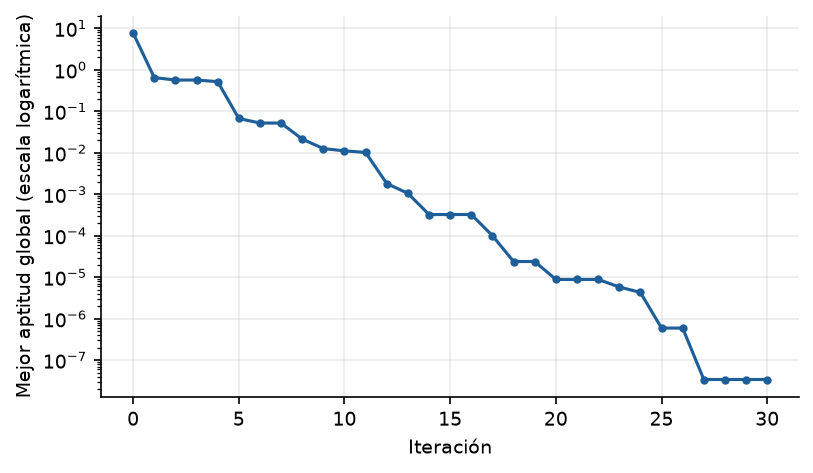
\includegraphics[width=0.85\textwidth]{p5_historial.png}
\caption{Mejor aptitud global por iteración en escala logarítmica.}
\label{fig:p5-historial}
\end{figure}
\comoleerla
{iteraciones en el eje horizontal y mejor aptitud global en el vertical, en
escala logarítmica.}
{una curva descendente con tramos planos.}
{los tramos planos son iteraciones sin mejora de $g_{best}$; la escala
logarítmica deja ver que la mejora sigue durante varios órdenes de magnitud.}

\begin{figure}[H]
\centering
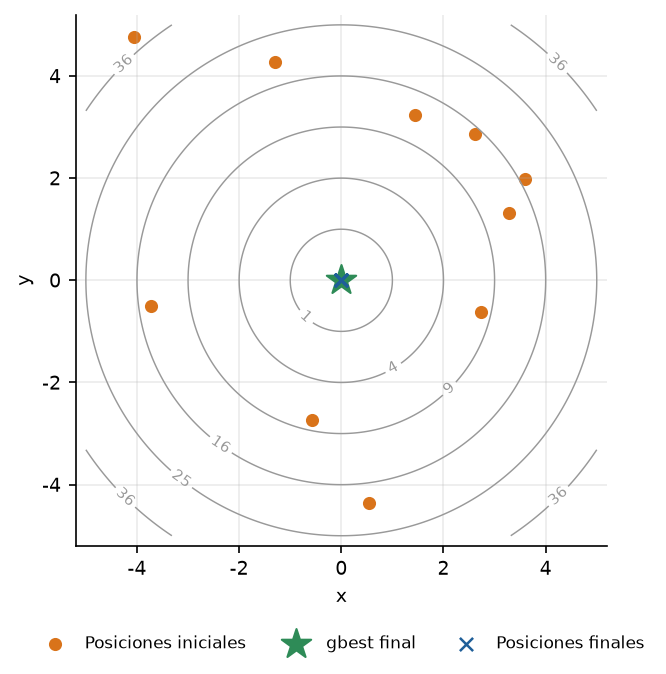
\includegraphics[width=\textwidth]{p5_curvas_nivel.png}
\caption{Curvas de nivel de $f(x,y)$ con las posiciones de las diez
partículas. Panel (a): dominio completo con su borde, las posiciones
iniciales numeradas, todas dentro de $[-5,5]^2$, y el $g_{best}$ final.
Panel (b): ampliación alrededor del origen con las posiciones finales y el
$g_{best}$.}
\label{fig:p5-curvas}
\end{figure}
\comoleerla
{dos paneles. En (a), círculos concéntricos que son las curvas de nivel
$f=1,4,9,16,25,36$, el borde discontinuo del dominio $[-5,5]^2$, puntos
naranjas numerados del 1 al 10 (posiciones iniciales) y una estrella verde
($g_{best}$). En (b), las mismas coordenadas ampliadas alrededor del origen,
con los ejes en unidades de la potencia de diez indicada, cruces azules
(posiciones finales) y la estrella verde hueca ($g_{best}$).}
{en (a), las diez posiciones iniciales están dentro del dominio y dispersas
en él. En (b), las diez cruces finales quedan a menos de \PcincoMaxFinal{} del
origen, con dos de ellas casi superpuestas junto a la estrella.}
{el panel (a) muestra que el enjambre parte de todo el dominio y el panel (b),
que la contracción hacia el mínimo es tan grande que solo se distingue a otra
escala.}

\subsubsection{Pregunta de interpretación}

\textbf{¿Por qué convergen sin alcanzar exactamente $(0,0)$?}
\begin{itemize}
  \item \textbf{Resultado obtenido.} El mejor punto es
  $(\PcincoX,\;\PcincoY)$, a \PcincoDist{} del origen, con
  $f=\PcincoF>0$.
  \item \textbf{Espacio continuo.} El dominio tiene infinitos puntos. Las
  partículas solo visitan los que genera la regla de movimiento, y es
  prácticamente imposible que alguna caiga exactamente en $(0,0)$.
  \item \textbf{$g_{best}$ es una posición muestreada.} Es el mejor punto
  que alguna partícula visitó, no el óptimo exacto. El término social atrae a
  todas hacia ese punto, no hacia $(0,0)$.
  \item \textbf{La velocidad decae pero no se anula.} Con $w=0{,}5$ la
  inercia se reduce a la mitad en cada paso, pero los términos cognitivo y
  social, multiplicados por números aleatorios, siguen aportando. Al
  terminar, la rapidez media es \PcincoRapidez{}, distinta de cero.
  \item \textbf{Iteraciones finitas.} Con 30 iteraciones el proceso se
  detiene antes de llegar más cerca. La última mejora ocurrió en la
  iteración \PcincoUltimaMejora{} y la mejora continuaba cerca del final.
  \item \textbf{Componente aleatoria.} Los valores de $r_1$ y $r_2$ cambian
  en cada paso, de modo que las partículas no se posan en un punto: la
  distancia media de las diez al origen es \PcincoDistMedia{}, mayor que la
  de $g_{best}$.
\end{itemize}

%=====================================================================
\section{Conclusiones}

\begin{itemize}
  \item \textbf{Algoritmo genético.} Con población de cuatro y elitismo, la
  mejor aptitud nunca bajó. El óptimo \PunoOptimo{} apareció en la generación
  \PunoPrimeraGen{}, después de una larga meseta, y solo gracias a una
  mutación: la población había perdido el único cuarto bit en $1$.
  \item \textbf{Ascenso de colinas.} Es determinista y su resultado depende
  del estado inicial. Llegó al máximo global desde \PdosExitos{} de
  \PdosTotal{} inicios. Con reinicios, la probabilidad de éxito sube a
  \PdosProbTres{} con tres y a \PdosProbCinco{} con cinco, sin llegar a $1$.
  \item \textbf{Temple simulado.} Aceptó \PtresPeores{} movimientos peores,
  todos en las primeras \PtresUltimoPeor{} iteraciones, y terminó en la mejor solución
  $x=\PtresMejor$. Guardar la mejor solución se justifica porque el estado
  actual estuvo peor que ella en \PtresPeorQueMejor{} iteraciones.
  \item \textbf{ACO.} La combinación de heurística y feromona llevó a las
  diez hormigas a $A$-$B$-$Z$ desde la iteración \PcuatroIterTodas{}. La
  convergencia fue rápida y dejó de explorar las otras rutas.
  \item \textbf{PSO.} El enjambre redujo la mejor aptitud de
  \PcincoFInicial{} a \PcincoF{}, a \PcincoDist{} del origen, sin alcanzarlo
  exactamente.
  \item \textbf{Exploración y explotación.} En los cinco métodos el equilibrio
  cambió con el tiempo. La mutación, la temperatura alta, la evaporación y la
  componente aleatoria sostienen la exploración; la selección, el enfriamiento,
  la feromona y $g_{best}$ concentran la búsqueda. Los resultados dependen de
  una sola semilla (42) y no deben generalizarse a todas las ejecuciones.
\end{itemize}

\end{document}
